%%%%%%%%%%%%%%%%%%%%%%%%%%%%%%%%%%%%%%%%%%%%%%%%%%%%%%%
%%%%%%%%%%%%%%%%%%%%%%%%%%%%%%%%%%%%%%%%%%%%%%%%%%%%%%%
%%
%Este template em \LaTeX\ foi desenvolvido pelo \textbf{Prof. Dr. José Wilker de Lima Silva} (UEPB) com o objetivo de facilitar a elaboração de trabalhos acadêmicos em conformidade com as %normas da ABNT. Além de fornecer uma estrutura organizada para monografias, dissertações e %teses, o template reúne exemplos dos principais recursos do \LaTeX, como capítulos, seções, %subseções, citações, figuras, tabelas, equações, listas, nomenclaturas, algoritmos e %referências bibliográficas. Sugestões, correções e melhorias são sempre bem-vindas e %contribuirão para o aperfeiçoamento contínuo deste material. Versão Julho/2026
%Contato: wilker+template@servidor.uepb.edu.br
%%
%%%%%%%%%%%%%%%%%%%%%%%%%%%%%%%%%%%%%%%%%%%%%%%%%%%%%%%
%---------------- PACOTES -----------------------------
%%%%%%%%%%%%%%%%%%%%%%%%%%%%%%%%%%%%%%%%%%%%%%%%%%%%%%%

\documentclass[12pt, a4paper]{report}

\usepackage{morewrites} % <-- Adicionado o mais alto possível!

% !TeX TXS-program:compile = txs:///pdflatex | txs:///makeindex %.nlo -s nomencl.ist -o %.nls | txs:///pdflatex

\usepackage{morewrites} % <-- Importante estar no topo da lista de pacotes!

%-------------------------------------------------------
% CONFIGURAÇÃO DA PÁGINA
%-------------------------------------------------------
\usepackage[top=3cm, bottom=2cm, right=2cm, left=3cm]{geometry} % Margens ABNT

%-------------------------------------------------------
% IDIOMA E CODIFICAÇÃO
%-------------------------------------------------------
\usepackage[utf8]{inputenc}      % Permite digitação em UTF-8 (acentuação)
\usepackage[brazilian]{babel}    % Traduz automaticamente nomes para o português
\usepackage{silence}
\WarningFilter{tracklang}{No `datatool' support for dialect}

%-------------------------------------------------------
% PDF
%-------------------------------------------------------
\usepackage[final]{pdfpages}     % Insere páginas de arquivos PDF

%-------------------------------------------------------
% CITAÇÕES, LEGENDAS E NUMERAÇÃO
%-------------------------------------------------------
\usepackage{csquotes}            % Aspas inteligentes
\usepackage[labelsep=endash]{caption} % Formatação das legendas de figuras e tabelas

% Desvincula a numeração de figuras e tabelas dos capítulos (1, 2, 3...)
\counterwithout{figure}{chapter}
\counterwithout{table}{chapter}

%-------------------------------------------------------
% PARÁGRAFOS
%-------------------------------------------------------
\usepackage{indentfirst}         % Indenta o primeiro parágrafo de cada seção

%-------------------------------------------------------
% AMBIENTES PERSONALIZADOS (Gráficos e Quadros)
%-------------------------------------------------------
\usepackage{newfloat}            % Permite criar novos ambientes flutuantes

\DeclareFloatingEnvironment[
    name=Gráfico, 
    listname={Lista de Gráficos},
    within=none % Garante numeração contínua (1, 2, 3...)
]{grafico}

\DeclareFloatingEnvironment[
    fileext=loq,
    listname={Lista de Quadros},
    name=Quadro,
    within=none % Garante numeração contínua (1, 2, 3...)
]{quadro}

%-------------------------------------------------------
% TEXTO DE EXEMPLO E APÊNDICES
%-------------------------------------------------------
\usepackage{blindtext}           % Gera texto fictício para testes
\usepackage{lipsum}              % Gera texto Lorem Ipsum
\usepackage[titletoc]{appendix}  % Melhor controle dos apêndices

% Altera o título da bibliografia
\addto{\captionsbrazil}{%
\renewcommand{\bibname}{\normalsize\bfseries\hfill REFERÊNCIAS\hfill}
}

%-------------------------------------------------------
% CABEÇALHO E NUMERAÇÃO DE PÁGINAS
%-------------------------------------------------------
\usepackage{fancyhdr}
\setlength{\headheight}{14.5pt} 

% Configura o estilo padrão para todas as páginas
\pagestyle{fancy}
\fancyhf{} % Limpa configurações antigas de cabeçalho e rodapé
\fancyhead[R]{\thepage} % Número da página no topo (Right/Direita)
\renewcommand{\headrulewidth}{0pt} % Remove a linha horizontal abaixo do número

% Redefine o estilo "plain" (usado automaticamente no início dos capítulos)
\fancypagestyle{plain}{
    \fancyhf{}
    \fancyhead[R]{\thepage}
    \renewcommand{\headrulewidth}{0pt}
}

\usepackage{epigraph}            % Cria epígrafes
\renewcommand{\textflush}{flushepinormal} % Alinhamento do texto da epígrafe

%-------------------------------------------------------
% FIGURAS E TABELAS
%-------------------------------------------------------
\usepackage{graphicx}            % Inclusão de imagens
\usepackage{float}               % Posicionamento preciso de figuras e tabelas (H)
\usepackage{capt-of}             % Permite usar legendas fora de ambientes flutuantes
\usepackage{booktabs}            % Tabelas com melhor qualidade tipográfica
\usepackage{longtable}           % Necessário para o glossário customizado

%-------------------------------------------------------
% DESENHOS E DIAGRAMAS
%-------------------------------------------------------
\usepackage{tikz}                % Desenhos vetoriais
\usetikzlibrary{arrows.meta,bending} % Bibliotecas extras do TikZ
\usepackage[all]{xy}             % Diagramas comutativos (matemática)

%-------------------------------------------------------
% MATEMÁTICA E FÍSICA
%-------------------------------------------------------
\usepackage{amsmath}             % Fórmulas matemáticas
\usepackage{amssymb}             % Símbolos matemáticos
\usepackage{amsfonts}            % Fontes matemáticas
\usepackage{amsthm}              % Ambientes de teoremas
\usepackage{MnSymbol}            % Símbolos matemáticos adicionais
\usepackage{thmtools}            % Gerenciamento avançado de teoremas
\usepackage{physics}             % Comandos úteis para Física e Matemática
\usepackage{cancel}              % Cancela termos em equações

\DeclareMathOperator{\mdc}{mdc}  % Operador matemático "mdc"
\DeclareMathOperator{\sen}{sen}  % Operador matemático "sen"

%-------------------------------------------------------
% TEXTO E CAIXAS
%-------------------------------------------------------
\usepackage{hyphenat}            % Controle da hifenização
\usepackage{setspace}            % Controle do espaçamento entre linhas
\linespread{1.25}                % Espaçamento de 1,25
\usepackage{boxedminipage}       % Cria caixas envolvendo blocos de texto
\usepackage{enumitem}            % Personalização de listas
\usepackage{changepage}          % Permite alterar margens temporariamente

\newenvironment{citacao}
{\begin{quote}\small\singlespacing}
{\{end{quote}}

%-------------------------------------------------------
% NOMENCLATURA E SIGLAS
%-------------------------------------------------------
\usepackage{nomencl}             % Lista de símbolos (nomenclatura)
\makenomenclature                % Inicializa o gerador de símbolos
\setlength{\nomlabelwidth}{3cm}
\setlength{\nomitemsep}{-\parsep}
\renewcommand{\nomname}{\normalsize \makebox[\linewidth]{\MakeUppercase{Lista de Símbolos}}}

\usepackage[acronym,nogroupskip]{glossaries}
\makeglossaries                  % Inicializa o gerador de siglas
\renewcommand{\glossarysection}[2][]{}

\newglossarystyle{siglasABNT}{
  \setglossarystyle{long}
  \renewenvironment{theglossary}
  {\begin{longtable}{@{}p{3cm}p{12cm}@{}}}
  {\end{longtable}}
  \renewcommand*{\glossentry}[2]{%
    \glstarget{##1}{\textbf{\glossentryname{##1}}} & \glossentrydesc{##1} \\
  }
}

\newcommand{\sigla}[2]{%
    \newacronym{#1}{#1}{#2}%
    \gls{#1}%
}

% --- DEFINIÇÃO DAS SIGLAS DO TRABALHO ---
\newacronym{etl}{ETL}{\textit{Extract, Transform and Load}}
\newacronym{elt}{ELT}{\textit{Extract, Load, Transform}}
\newacronym{ssis}{SSIS}{SQL Server Integration Services}
\newacronym{dag}{DAG}{\textit{Directed Acyclic Graph}}
\newacronym{sefazpb}{SEFAZ-PB}{Secretaria de Estado da Fazenda da Paraíba}
\newacronym{atf}{ATF}{Sistema de Administração Tributária e Financeira}
\newacronym{sor}{SOR}{\textit{System of Record}}
\newacronym{scamf}{SCAMF}{Sistema de Controle e Análise das Malhas Fiscais}
\newacronym{nfe}{NFe}{Nota Fiscal Eletrônica}
\newacronym{nfce}{NFCe}{Nota Fiscal de Consumidor Eletrônica}
\newacronym{cte}{CTe}{Conhecimento de Transporte Eletrônico}
\newacronym{efd}{EFD}{Escrituração Fiscal Digital}
\newacronym{bi}{BI}{\textit{Business Intelligence}}
\newacronym{nutes}{Nutes}{Núcleo de Tecnologia Estratégica em Saúde}
\newacronym{ufpb}{UFPB}{Universidade Federal da Paraíba}

%-------------------------------------------------------
% DATAS E TÍTULOS DE SEÇÃO
%-------------------------------------------------------
\usepackage{datetime}
\usepackage{titlesec}

\titleformat*{\section}{\normalsize \bfseries}
\titleformat*{\subsection}{\normalsize\itshape\bfseries}
\titleformat*{\subsubsection}{\normalsize \bfseries}
\titleformat*{\paragraph}{\large\bfseries}
\titleformat*{\subparagraph}{\large\bfseries}
\titleformat{\chapter}{\bfseries}{\filright \thechapter}{20pt}{\filright}
\titlespacing*{\chapter}{0pt}{0pt}{*1.5}
\titlespacing{\section}{0pt}{*1.5}{*1.5}

%-------------------------------------------------------
% TOCLOFT: FORMATAÇÃO DO SUMÁRIO (ABNT NBR 6027: 2012)
%-------------------------------------------------------
\usepackage{tocloft}

\renewcommand\cftchapnumwidth{3.8em}
\renewcommand\cftsecnumwidth{3.8em}
\renewcommand\cftsubsecnumwidth{3.8em}
\renewcommand{\cftsecfont}{\bfseries }

\renewcommand{\cftfigpresnum}{Figura~}
\renewcommand{\cftfigaftersnum}{ --}
\settowidth{\cftfignumwidth}{Figura 99 --}

\renewcommand{\cfttabpresnum}{Tabela~}
\renewcommand{\cfttabaftersnum}{ --}
\settowidth{\cfttabnumwidth}{Tabela 99 --}

% Configurações para a Lista de Quadros
\newlength{\cftquadnumwidth}
\newcommand{\cftquadpresnum}{Quadro~}
\newcommand{\cftquadaftersnum}{ --}
\settowidth{\cftquadnumwidth}{\cftquadpresnum 99\cftquadaftersnum}

% Configurações para a Lista de Gráficos
\newlength{\cftgrafnumwidth}
\newcommand{\cftgrafpresnum}{Gráfico~}
\newcommand{\cftgrafaftersnum}{ --}
\settowidth{\cftgrafnumwidth}{\cftgrafpresnum 99\cftgrafaftersnum}

% Atalhos de referência
\newcommand{\tabref}[1]{Tabela~\ref{#1}}
\newcommand{\figref}[1]{Figura~\ref{#1}}
\newcommand{\secref}[1]{Seção~\ref{#1}}
\newcommand{\chapref}[1]{Capítulo~\ref{#1}}
\newcommand{\eqnref}[1]{Equação~\eqref{#1}}

% Recuos de seção
\setlength{\cftsecindent}{0pt}
\setlength{\cftsubsecindent}{0pt}

% Formatação do título do sumário e listas
\renewcommand{\cfttoctitlefont}{\hfil \normalfont \centering \bfseries\MakeUppercase}
\renewcommand{\cftaftertoctitle}{\\[\baselineskip]\mbox{}\hfill{\normalfont Página}}
\setlength{\cftbeforetoctitleskip}{-1.5em}
\setlength{\cftaftertoctitleskip}{0pt}

%-------------------------------------------------------
% AMBIENTES DE TEOREMAS E APLICAÇÕES
%-------------------------------------------------------
\newtheorem{theorem}{Teorema}[chapter]
\newtheorem{teorema}{Teorema}[chapter]
\newtheorem{corollary}{Corolário}[theorem]
\newtheorem{corolario}{Corolário}[chapter]
\newtheorem{lemma}[theorem]{Lema}

\theoremstyle{remark}
\newtheorem{remark}{Observação}[chapter]

\theoremstyle{definition}
\newtheorem{definition}{Definição}[chapter]
\newtheorem{exemplo}{Exemplo}[chapter]

\theoremstyle{plain}
\newtheorem{lema}{Lema}[chapter]
\newtheorem{prop}{Proposição}[chapter]
\newtheorem{cor}{Corolário}[chapter]

\declaretheorem[style=definition,qed=$\filledmedtriangleleft$, name=Aplicação, numberwithin=chapter]{ap}

\theoremstyle{definition}
\newtheorem*{nota}{Notação}

%-------------------------------------------------------
% INJEÇÃO DOS PREFIXOS NAS LISTAS (Gráfico e Quadro)
%-------------------------------------------------------
\makeatletter
% Formatação da Lista de Gráficos
\renewcommand{\l@grafico}[2]{%
  \begingroup
  \renewcommand{\numberline}[1]{\hb@xt@\@tempdima{\cftgrafpresnum##1\cftgrafaftersnum\hfil}}%
  \@dottedtocline{1}{0em}{\cftgrafnumwidth}{#1}{#2}%
  \endgroup
}

% Formatação da Lista de Quadros
\renewcommand{\l@quadro}[2]{%
  \begingroup
  \renewcommand{\numberline}[1]{\hb@xt@\@tempdima{\cftquadpresnum##1\cftquadaftersnum\hfil}}%
  \@dottedtocline{1}{0em}{\cftquadnumwidth}{#1}{#2}%
  \endgroup
}

% Comandos nativos para geração de listas pelo sumário global
\renewcommand{\listoffigures}{\@starttoc{lof}}
\renewcommand{\listoftables}{\@starttoc{lot}}
\makeatother

%-------------------------------------------------------
% REFERÊNCIAS CRUZADAS E LINKS
%-------------------------------------------------------
\usepackage[
    colorlinks=true, % Ativa cores nos links
    linkcolor=black, % Cor dos links internos
    citecolor=black, % Cor dos links das citações bibliográficas
    urlcolor=black   % Cor dos links de internet
]{hyperref}

%-------------------------------------------------------
% CITAÇÕES ABNT E BACKREF
%-------------------------------------------------------
\usepackage[brazilian,hyperpageref]{backref}
\usepackage[alf]{abntex2cite}

% Configurações do pacote backref
\renewcommand{\backrefpagesname}{Citada na(s) página(s):~}
\renewcommand{\backref}{}
\renewcommand*{\backrefalt}[4]{
    \ifcase #1 %
        Nenhuma citação no texto.%
    \or
        Citação na pág. #2.%
    \else
        Citação nas págs. #2.%
    \fi}

%Adicionados por mim
\usepackage{array}
\usepackage{tabularx}

\begin{document}

\nocite{minha-opcao-de-citacao}

%%%%%%%%%%%%%%%%%%%%%%%%%%%%%%%%%%%%%%%%%%%%%%%%%%%%%%%
%---------- CONFIGURAÇÃO DO TRABALHO ------------------
%%%%%%%%%%%%%%%%%%%%%%%%%%%%%%%%%%%%%%%%%%%%%%%%%%%%%%%

% Tipo de trabalho:
% 1 = Trabalho de Conclusão de Curso
% 2 = Dissertação
% 3 = Tese
\newcommand{\tipodetrabalhonum}{1} % <-- Altere apenas este número

% Nome do tipo de trabalho
\newcommand{\tipodetrabalho}{%
\ifcase\tipodetrabalhonum
\or Trabalho de Conclusão de Curso%
\or Dissertação%
\or Tese%
\else Tipo de trabalho inválido%
\fi
}

% Grau obtido
\newcommand{\grau}{%
\ifcase\tipodetrabalhonum
\or Bacharel(a) / Licenciado(a) / Tecnólogo(a) % <-- Editar apenas para TCC
\or Mestre(a)%
\or Doutor(a)%
\else Grau inválido%
\fi
}

%%%%%%%%%%%%%%%%%%%%%%%%%%%%%%%%%%%%%%%%%%%%%%%%%%%%%%%
%---------- DADOS INSTITUCIONAIS ----------------------
%%%%%%%%%%%%%%%%%%%%%%%%%%%%%%%%%%%%%%%%%%%%%%%%%%%%%%%

\newcommand{\universidade}{Universidade Estadual da Paraíba}
\newcommand{\siglauniversidade}{UEPB}

\newcommand{\campus}{CAMPUS I - CAMPINA GRANDE}

\newcommand{\proreitoria}{%
PRÓ-REITORIA DE PÓS-GRADUAÇÃO E PESQUISA}

\newcommand{\centro}{%
Centro de Ciências e Tecnologia}

\newcommand{\departamentoouprograma}{%
Departamento de Ciência de Dados}

\newcommand{\coordenacao}{%
Coordenação do Curso de Ciência de Dados}

\newcommand{\curso}{%
Curso de Ciência de Dados}

\newcommand{\nomedocurso}{%
Ciência de Dados}

%%%%%%%%%%%%%%%%%%%%%%%%%%%%%%%%%%%%%%%%%%%%%%%%%%%%%%%
%---------- DADOS DO TRABALHO -------------------------
%%%%%%%%%%%%%%%%%%%%%%%%%%%%%%%%%%%%%%%%%%%%%%%%%%%%%%%

\newcommand{\titulo}{Título do Trabalho}

\newcommand{\area}{%
Qualidade de Sistemas Ambientais}

\newcommand{\cidade}{%
CAMPINA GRANDE - PB}

\newcommand{\datadeaprovacao}{01/01/2000}

%%%%%%%%%%%%%%%%%%%%%%%%%%%%%%%%%%%%%%%%%%%%%%%%%%%%%%%
%---------- DADOS DO(A) AUTOR(A) ----------------------
%%%%%%%%%%%%%%%%%%%%%%%%%%%%%%%%%%%%%%%%%%%%%%%%%%%%%%%

\newcommand{\estudante}{Nome do(a) Estudante(a)}

%%%%%%%%%%%%%%%%%%%%%%%%%%%%%%%%%%%%%%%%%%%%%%%%%%%%%%%
%---------- ORIENTAÇÃO --------------------------------
%%%%%%%%%%%%%%%%%%%%%%%%%%%%%%%%%%%%%%%%%%%%%%%%%%%%%%%

\newcommand{\orientador}{Prof. Dr(a). Fulano de Tal}

%%%%%%%%%%%%%%%%%%%%%%%%%%%%%%%%%%%%%%%%%%%%%%%%%%%%%%%
%---------- BANCA EXAMINADORA -------------------------
%%%%%%%%%%%%%%%%%%%%%%%%%%%%%%%%%%%%%%%%%%%%%%%%%%%%%%%

% Membro 1
\newcommand{\membrob}{Prof. Dr. B}
\newcommand{\filiacaob}{Universidade Federal}
\newcommand{\siglafiliacaob}{UFB}

% Membro 2
\newcommand{\membroc}{Prof. Dr. C}
\newcommand{\filiacaoc}{Universidade Estadual}
\newcommand{\siglafiliacaoc}{UEC}

% Membro 3 (utilizado apenas quando necessário)
\newcommand{\membrod}{Prof. Dr. D}
\newcommand{\filiacaod}{Instituto Federal}
\newcommand{\siglafiliacaod}{IFD}

% Membro 4 (utilizado apenas quando necessário)
\newcommand{\membroe}{Prof. Dr. E}
\newcommand{\filiacaoe}{Universidade Estadual}
\newcommand{\siglafiliacaoe}{UEE}

%%%%%%%%%%%%%%%%%%%%%%%%%%%%%%%%%%%%%%%%%%%%%%%%%%%%%%%

%Pré-Textual
%---CAPA

\begin{titlepage}
\begin{center}
\begin{figure}
    \centering
    
\includegraphics[height=!, width= 2cm]{config/logo-uepb.png}
\end{figure}

\textbf{
\MakeUppercase\universidade\\
\MakeUppercase\campus\\
\ifnum\tipodetrabalhonum>1
\MakeUppercase\proreitoria\\
\fi
\MakeUppercase\centro\\
\MakeUppercase\departamentoouprograma\\
\MakeUppercase\curso
}

\vspace{4cm}


\textbf{\MakeUppercase\estudante}   

\vspace{4cm}
\textbf{\MakeUppercase\titulo}

\vfill

\textbf{\MakeUppercase\cidade\\
\the\year} 
    
\end{center}
\end{titlepage}

% Inicia a contagem na folha de rosto
\clearpage
\pagenumbering{arabic}
\setcounter{page}{1}

% Não mostra o número nas páginas pré-textuais
\pagestyle{empty}
%----------------
%--FOLHA DE ROSTO

\thispagestyle{empty}
\begin{center}
 
    
\textbf{\MakeUppercase\estudante}    

\vspace{5cm}

\textbf{\MakeUppercase\titulo}   

\vspace{5cm}

\begin{flushright}
\parbox{8cm}{
\singlespacing{\begin{hyphenrules}{nohyphenation}
\tipodetrabalho~apresentada à \coordenacao \ da \universidade, como requisito parcial à obtenção do título de \grau \ em \nomedocurso. % natureza do trabalho
\vspace{0.5cm}    

\textbf{Área de concentração}: \area
\end{hyphenrules}}}
\end{flushright}


\vspace{2cm}

\textbf{Orientador}: \orientador
\vfill


\textbf{CAMPINA GRANDE - PB\\
\the\year}
\end{center}
\newpage % Comentar esta linha e liberar a linha abaixo caso queira inserir pdf com folha de rosto
% A ficha catalográfica deve ficar no verso da folha de rosto.
% Se estiver incluindo em um projeto maior (book/report), 
% use \newpage ou \clearpage antes deste bloco.
\thispagestyle{empty}

% Joga o conteúdo da ficha para o final (rodapé) da página
\vspace*{\fill}

\begin{center}
    \small
    É expressamente proibida a comercialização deste documento, tanto na forma impressa como eletrônica. 
    Sua reprodução total ou parcial é permitida exclusivamente para fins acadêmicos e científicos, 
    desde que na reprodução figure a identificação do autor, título, instituição e ano da defesa.
    
    \vspace{1cm}
    
    \textbf{Ficha Catalográfica elaborada pela Biblioteca da Universidade Estadual da Paraíba}
    
    \vspace{0.5cm}
    
    % Caixa retangular padrão de fichas catalográficas
    \fbox{
        \begin{minipage}[c][8.5cm]{13.5cm}
            \vspace{0.5cm}
            % Coluna do código de catalogação (Cutter)
            \begin{minipage}[t]{1.5cm}
                S000x
            \end{minipage}%
            % Coluna com os dados bibliográficos
            \begin{minipage}[t]{11.5cm}
                \singlespacing
                Sobrenome, Nome do Autor.\\
                \hspace*{0.5cm} Título do trabalho acadêmico: subtítulo (se houver) / Nome do Autor. -- Campina Grande, 2026.\\
                \hspace*{0.5cm} 120 f. : il. color.\\
                \\
                \hspace*{0.5cm} Orientador: Prof. Dr. Nome do Orientador.\\
                \hspace*{0.5cm} Coorientador: Prof. Dr. Nome do Coorientador (se houver).\\
                \\
                \hspace*{0.5cm} Trabalho de Conclusão de Curso (Graduação em [Nome do Curso]) -- Universidade Estadual da Paraíba, Centro de [Nome do Centro], [Ano da defesa].\\
                \\
                \hspace*{0.5cm} 1. Primeira palavra-chave. 2. Segunda palavra-chave. 3. Terceira palavra-chave. I. Título.
                
                \vspace{0.5cm}
                % Código Dewey Decimal Classification (CDD) ou CDU
                \begin{flushright}
                    \textbf{CDD} 000.000
                \end{flushright}
            \end{minipage}
            \vspace*{0.2cm}
        \end{minipage}
    }
\end{center}

\newpage %<---- trocar pelo pdf da ficha catalografica
%\includepdf{pre-textual/fichacatalografica.pdf} %<--- Liberar essa linha para inserir outra ficha
%----------------
%--FOLHA DE APROVAÇÃO

\thispagestyle{empty}
\begin{center}
\textbf{\MakeUppercase\estudante}

\vspace{1cm}

\textbf{\MakeUppercase\titulo}

\end{center}

\vspace{.4cm}
\begin{flushright}
\parbox{8cm}{
\singlespacing{\begin{hyphenrules}{nohyphenation}
\tipodetrabalho~apresentada à \coordenacao \ da \universidade, como requisito parcial à obtenção do título de \grau \ em \nomedocurso. % natureza do trabalho
\vspace{0.5cm}

\textbf{Área de concentração}: \area
\end{hyphenrules}}}
\end{flushright}

\vspace{.6cm}

\noindent Aprovado em: \datadeaprovacao     %<----- Inserir data no estilo dd/mm/aaaa

\begin{center}

\textbf{BANCA EXAMINADORA}

\vspace{0.8cm}

%-----------------------------------
% Orientador (sempre aparece)
%-----------------------------------

\noindent\rule{12cm}{0.4pt}\\
\orientador\ \ (Orientador(a))\\
\universidade\ (\siglauniversidade)

\vspace{0.5cm}

%-----------------------------------
% Membro B (sempre aparece)
%-----------------------------------

\noindent\rule{12cm}{0.4pt}\\
\membrob\\
\filiacaob\ (\siglafiliacaob)

\vspace{0.5cm}

%-----------------------------------
% Membro C (sempre aparece)
%-----------------------------------

\noindent\rule{12cm}{0.4pt}\\
\membroc\\
\filiacaoc\ (\siglafiliacaoc)

\vspace{0.5cm}

%-----------------------------------
% Apenas Dissertação e Tese
%-----------------------------------

\ifnum\tipodetrabalhonum>1

\noindent\rule{12cm}{0.4pt}\\
\membrod\\
\filiacaod\ (\siglafiliacaod)

\vspace{0.5cm}

\noindent\rule{12cm}{0.4pt}\\
\membroe\\
\filiacaoe\ (\siglafiliacaoe)

\vspace{0.5cm}

\fi

\end{center}%<--- COMENTAR SE usar PDF
%\includepdf{pre-textual/folhadeaprovacao.pdf} %<--- Liberar essa linha para inserir outra folha de aprovacao
%--------------
%---DEDICATÓRIA
\newpage
\thispagestyle{empty}
\null
\vfill
\begin{flushright}
\parbox{4cm}{
\singlespacing{\begin{hyphenrules}{nohyphenation}
Dedico este trabalho a Deus, por sua constante presença em minha caminhada, 
e aos meus pais, pelo amor, apoio, dedicação e incentivo em todos os momentos.
\end{hyphenrules}
}}
\end{flushright}
\thispagestyle{empty}
\newpage
%-----------------
%---AGRADECIMENTOS

\thispagestyle{empty}
\section*{\normalsize \centering \textbf{AGRADECIMENTOS}}

Agradeço, primeiramente, a Deus, por me conceder força, perseverança e sabedoria para chegar até aqui.

Aos meus pais, Alexandre e Anamercia, agradeço por todo o apoio, incentivo, compreensão e por sempre 
acreditarem em mim. Esta conquista também é de vocês.

Ao meu orientador, Fábio Luiz Leite Júnior, agradeço pela orientação, disponibilidade, paciência e 
pelos ensinamentos ao longo do desenvolvimento deste trabalho, que contribuíram para minha formação 
acadêmica e profissional.

Aos meus colegas de equipe, agradeço pela parceria, colaboração e ajuda durante o desenvolvimento do 
projeto. Em especial, agradeço a Lucas Maia e Alisson Otavio, que contribuíram diretamente para o 
desenvolvimento do trabalho, auxiliando em diferentes etapas e compartilhando seus conhecimentos. 
Agradeço também aos colaboradores da UFPB, especialmente ao Prof. Marcelo Iury, pelas 
contribuições, disponibilidade e interações que foram importantes para o desenvolvimento do projeto, 
especialmente nas atividades relacionadas ao Data Lake.

Aos meus amigos e demais colegas, agradeço pela companhia, pelas conversas, pelo apoio e pelos momentos 
compartilhados ao longo dessa caminhada.

Por fim, agradeço a todos que, direta ou indiretamente, contribuíram para a realização deste trabalho 
e para que eu chegasse até aqui.

\newpage
%%-----------
%---EPÍGRAFE

\thispagestyle{empty}

\vspace*{\fill}

\begin{flushright}
\begin{minipage}{8cm}

\enquote{Citação relacionada com o tema do trabalho, com indicação de autoria.}

\vspace{0.5cm}

--- Autor(a)

\end{minipage}
\end{flushright}

\newpage
%---------
%---RESUMO

\thispagestyle{empty}
\section*{\normalsize \centering \textbf{RESUMO}}

\noindent  

Este trabalho aborda a modernização dos processos de Extração, Transformação e Carga (ETL) da Secretaria de Estado da 
Fazendada Paraíba (SEFAZ-PB), motivada pelas limitações da arquitetura legada baseada em SQL Server Integration 
Services (SSIS) frente às demandas dos ambientes de Big Data. Nesse contexto, o estudo teve como objetivo propor 
uma reestruturação da estratégia de ETL da SEFAZ-PB, utilizando o projeto BDMalhas como estudo de caso. Para isso, 
foi desenvolvido um novo sistema de ETL baseado em Apache Airflow, Apache Spark e ClickHouse, cuja avaliação 
considerou métricas de manutenibilidade, desempenho e utilização de espaço em disco, além da análise dos desafios 
e limitações da reestruturação. Para tanto, a pesquisa foi conduzida como um estudo de caso, de caráter aplicado 
e abordagem quantitativa, envolvendo a implementação da arquitetura proposta e sua avaliação por meio de 
experimentos comparativos. Ao final, os resultados evidenciaram redução da complexidade estrutural dos pipelines, 
do tempo de execução das cargas e do espaço em disco utilizado, além de ganhos em manutenibilidade e escalabilidade.
Por outro lado, também foram identificados desafios, destacando-se a migração da arquitetura legada e as limitações 
do ambiente experimental. Por fim, conclui-se que a reestruturação proposta constitui uma alternativa viável para 
modernizar os processos de ETL da SEFAZ-PB, proporcionando ganhos em desempenho, manutenibilidade e escalabilidade, 
embora os resultados estejam restritos ao contexto do projeto BDMalhas e ao ambiente utilizado na pesquisa.

\vspace*{0.5cm}

\noindent\textbf{Palavras-chave:} ETL; Big Data; engenharia de dados; reestruturação de ETL; arquitetura de dados.
 % no máximo 4 palavras-chave separadas entre si por ponto 
 \newpage

%---------
%---ABSTRACT

\thispagestyle{empty}
\section*{\normalsize \centering \textbf{ABSTRACT}}

\noindent This \LaTeX\ template was developed by \textbf{Prof. Dr. José Wilker de Lima Silva} (UEPB) with the aim of facilitating the preparation of academic works in compliance with ABNT standards. Besides providing a structured framework for undergraduate monographs, master's dissertations, and doctoral theses, the template presents examples of the main resources available in \LaTeX, including chapters, sections, subsections, citations, figures, tables, equations, lists, nomenclature, algorithms, and bibliographic references. Suggestions, corrections, and contributions for improvement are highly appreciated and will support the continuous refinement of this material.

\vspace*{0.5cm}

\noindent\textbf{Keywords:} keyword 1. keyword 2. keyword 3.
\newpage
%----------
%---LISTAS DE FIGURAS, TABELAS, QUADROS E SÍMBOLOS
% OBS: NÃO FAZER EDIÇÕES NESTE ARQUIVO pre-textual/10-listas ********************
% =======================================================
% CONFIGURAÇÕES E IMPRESSÃO DAS LISTAS (TUDO EM UM ARQUIVO)
% Pode ser chamado com % =======================================================
% CONFIGURAÇÕES E IMPRESSÃO DAS LISTAS (TUDO EM UM ARQUIVO)
% Pode ser chamado com % =======================================================
% CONFIGURAÇÕES E IMPRESSÃO DAS LISTAS (TUDO EM UM ARQUIVO)
% Pode ser chamado com \input{listas} APÓS o \begin{document}
	% =======================================================
	
	\makeatletter
	
	%------------------------------------------------------------
	% 1. AJUSTES DO SUMÁRIO
	%------------------------------------------------------------
	\renewcommand{\cftsubsecfont}{\itshape\bfseries}
	\renewcommand{\cftsubsecpagefont}{\normalfont}
	
	%------------------------------------------------------------
	% 2. AJUSTES DOS PREFIXOS DAS LISTAS
	%------------------------------------------------------------
	\@ifundefined{cftfigpresnum}{}{
		\renewcommand{\cftfigpresnum}{\figurename~}
		\renewcommand{\cftfigaftersnum}{~--~}
		\settowidth{\cftfignumwidth}{\cftfigpresnum 000~--~}
	}
	\@ifundefined{cfttabpresnum}{}{
		\renewcommand{\cfttabpresnum}{\tablename~}
		\renewcommand{\cfttabaftersnum}{~--~}
		\settowidth{\cfttabnumwidth}{\cfttabpresnum 000~--~}
	}
	\@ifundefined{cftquadropresnum}{}{
		\renewcommand{\cftquadropresnum}{Quadro~}
		\renewcommand{\cftquadroaftersnum}{~--~}
		\settowidth{\cftquadronumwidth}{\cftquadropresnum 000~--~}
	}
	\@ifundefined{cftgraficopresnum}{}{
		\renewcommand{\cftgraficopresnum}{Gráfico~}
		\renewcommand{\cftgraficoaftersnum}{~--~}
		\settowidth{\cftgraficonumwidth}{\cftgraficopresnum 000~--~}
	}
	
	%------------------------------------------------------------
	% 3. REGISTRO E DETECÇÃO AUTOMÁTICA DE ELEMENTOS NO TEXTO
	%------------------------------------------------------------
	\let\native@addcontentsline\addcontentsline
	\renewcommand{\addcontentsline}[3]{%
		\immediate\write\@mainaux{\string\gdef\string\temitem@#1{1}}%
		\native@addcontentsline{#1}{#2}{#3}%
	}
	
	% Travas lógicas para escrever no .aux apenas 1 vez e evitar loops
	\def\temitem@acr@written{0}
	\newcommand{\RegistrarUsoAcr}{%
		\ifnum\temitem@acr@written=0
		\immediate\write\@mainaux{\string\gdef\string\temitem@acr{1}}%
		\global\def\temitem@acr@written{1}%
		\fi
	}
	
	\def\temitem@nls@written{0}
	\newcommand{\RegistrarUsoNls}{%
		\ifnum\temitem@nls@written=0
		\immediate\write\@mainaux{\string\gdef\string\temitem@nls{1}}%
		\global\def\temitem@nls@written{1}%
		\fi
	}
	
	% Monitora os comandos padrões do glossaries e o SEU comando customizado \sigla
	\@ifpackageloaded{glossaries}{
		\AddToHook{cmd/glsadd/before}{\RegistrarUsoAcr}
		\AddToHook{cmd/gls/before}{\RegistrarUsoAcr}
	}{}
	% Gatilho crucial para quem usa o comando \sigla{}{}:
	\AddToHook{cmd/sigla/before}{\RegistrarUsoAcr}
	
	\@ifpackageloaded{nomencl}{
		\AddToHook{cmd/nomenclature/before}{\RegistrarUsoNls}
	}{}
	
	\newcommand{\SeTemItem}[2]{%
		\def\elemento@achado{0}%
		\@ifundefined{temitem@#1}{}{%
			\def\elemento@achado{1}%
		}%
		\@ifundefined{ext@#1}{}{%
			\@ifundefined{temitem@\csname ext@#1\endcsname}{}{%
				\def\elemento@achado{1}%
			}%
		}%
		\ifnum\elemento@achado=1\relax
		#2%
		\fi
	}
	
	%------------------------------------------------------------
	% 4. LISTAS SEM TÍTULO AUTOMÁTICO E FORMATAÇÃO
	%------------------------------------------------------------
	\renewcommand{\listoffigures}{\@starttoc{lof}}
	\renewcommand{\listoftables}{\@starttoc{lot}}
	\renewcommand{\listof}[2]{\@starttoc{\csname ext@#1\endcsname}}
	
	\newcommand{\PreTextualTitulo}[1]{%
		\begin{center}
			\bfseries\MakeUppercase{#1}
		\end{center}
	}
	
	\makeatother
	
	% =======================================================
	% 5. IMPRESSÃO DAS LISTAS E SUMÁRIO
	% =======================================================
	
	% LISTA DE ILUSTRAÇÕES
	\SeTemItem{lof}{%
		\PreTextualTitulo{Lista de Ilustrações}
		\listoffigures
		\thispagestyle{empty}
		\newpage
	}
	
	% LISTA DE TABELAS
	\SeTemItem{lot}{%
		\PreTextualTitulo{Lista de Tabelas}
		\listoftables
		\thispagestyle{empty}
		\newpage
	}
	
	% LISTA DE ABREVIATURAS E SIGLAS
	\SeTemItem{acr}{%
		% Trava de segurança extra para garantir que não haja registros durante a impressão
		\global\def\temitem@acr@written{1}
		\PreTextualTitulo{Lista de Abreviaturas e Siglas}
		\printglossary[
		type=\acronymtype,
		style=siglasABNT,
		title={}
		]
		\thispagestyle{empty}
		\newpage
	}
	
	% LISTA DE SÍMBOLOS
	\SeTemItem{nls}{%
		\global\def\temitem@nls@written{1}
		\printnomenclature
		\thispagestyle{empty}
		\newpage
	}
	
	% LISTA DE QUADROS
	\SeTemItem{quadro}{%
		\PreTextualTitulo{Lista de Quadros}
		\listof{quadro}{}
		\thispagestyle{empty}
		\newpage
	}
	
	% LISTA DE GRÁFICOS
	\SeTemItem{grafico}{%
		\PreTextualTitulo{Lista de Gráficos}
		\listof{grafico}{}
		\thispagestyle{empty}
		\newpage
	}
	
	% SUMÁRIO
	\tableofcontents
	\thispagestyle{empty}
	
	% =======================================================
	% 6. CORREÇÃO DOS CONTADORES (ABNT)
	% =======================================================
	\setcounter{table}{0}
	\setcounter{figure}{0}
	\makeatletter
	\@ifundefined{c@quadro}{}{\setcounter{quadro}{0}}
	\@ifundefined{c@grafico}{}{\setcounter{grafico}{0}}
	\makeatother APÓS o \begin{document}
	% =======================================================
	
	\makeatletter
	
	%------------------------------------------------------------
	% 1. AJUSTES DO SUMÁRIO
	%------------------------------------------------------------
	\renewcommand{\cftsubsecfont}{\itshape\bfseries}
	\renewcommand{\cftsubsecpagefont}{\normalfont}
	
	%------------------------------------------------------------
	% 2. AJUSTES DOS PREFIXOS DAS LISTAS
	%------------------------------------------------------------
	\@ifundefined{cftfigpresnum}{}{
		\renewcommand{\cftfigpresnum}{\figurename~}
		\renewcommand{\cftfigaftersnum}{~--~}
		\settowidth{\cftfignumwidth}{\cftfigpresnum 000~--~}
	}
	\@ifundefined{cfttabpresnum}{}{
		\renewcommand{\cfttabpresnum}{\tablename~}
		\renewcommand{\cfttabaftersnum}{~--~}
		\settowidth{\cfttabnumwidth}{\cfttabpresnum 000~--~}
	}
	\@ifundefined{cftquadropresnum}{}{
		\renewcommand{\cftquadropresnum}{Quadro~}
		\renewcommand{\cftquadroaftersnum}{~--~}
		\settowidth{\cftquadronumwidth}{\cftquadropresnum 000~--~}
	}
	\@ifundefined{cftgraficopresnum}{}{
		\renewcommand{\cftgraficopresnum}{Gráfico~}
		\renewcommand{\cftgraficoaftersnum}{~--~}
		\settowidth{\cftgraficonumwidth}{\cftgraficopresnum 000~--~}
	}
	
	%------------------------------------------------------------
	% 3. REGISTRO E DETECÇÃO AUTOMÁTICA DE ELEMENTOS NO TEXTO
	%------------------------------------------------------------
	\let\native@addcontentsline\addcontentsline
	\renewcommand{\addcontentsline}[3]{%
		\immediate\write\@mainaux{\string\gdef\string\temitem@#1{1}}%
		\native@addcontentsline{#1}{#2}{#3}%
	}
	
	% Travas lógicas para escrever no .aux apenas 1 vez e evitar loops
	\def\temitem@acr@written{0}
	\newcommand{\RegistrarUsoAcr}{%
		\ifnum\temitem@acr@written=0
		\immediate\write\@mainaux{\string\gdef\string\temitem@acr{1}}%
		\global\def\temitem@acr@written{1}%
		\fi
	}
	
	\def\temitem@nls@written{0}
	\newcommand{\RegistrarUsoNls}{%
		\ifnum\temitem@nls@written=0
		\immediate\write\@mainaux{\string\gdef\string\temitem@nls{1}}%
		\global\def\temitem@nls@written{1}%
		\fi
	}
	
	% Monitora os comandos padrões do glossaries e o SEU comando customizado \sigla
	\@ifpackageloaded{glossaries}{
		\AddToHook{cmd/glsadd/before}{\RegistrarUsoAcr}
		\AddToHook{cmd/gls/before}{\RegistrarUsoAcr}
	}{}
	% Gatilho crucial para quem usa o comando \sigla{}{}:
	\AddToHook{cmd/sigla/before}{\RegistrarUsoAcr}
	
	\@ifpackageloaded{nomencl}{
		\AddToHook{cmd/nomenclature/before}{\RegistrarUsoNls}
	}{}
	
	\newcommand{\SeTemItem}[2]{%
		\def\elemento@achado{0}%
		\@ifundefined{temitem@#1}{}{%
			\def\elemento@achado{1}%
		}%
		\@ifundefined{ext@#1}{}{%
			\@ifundefined{temitem@\csname ext@#1\endcsname}{}{%
				\def\elemento@achado{1}%
			}%
		}%
		\ifnum\elemento@achado=1\relax
		#2%
		\fi
	}
	
	%------------------------------------------------------------
	% 4. LISTAS SEM TÍTULO AUTOMÁTICO E FORMATAÇÃO
	%------------------------------------------------------------
	\renewcommand{\listoffigures}{\@starttoc{lof}}
	\renewcommand{\listoftables}{\@starttoc{lot}}
	\renewcommand{\listof}[2]{\@starttoc{\csname ext@#1\endcsname}}
	
	\newcommand{\PreTextualTitulo}[1]{%
		\begin{center}
			\bfseries\MakeUppercase{#1}
		\end{center}
	}
	
	\makeatother
	
	% =======================================================
	% 5. IMPRESSÃO DAS LISTAS E SUMÁRIO
	% =======================================================
	
	% LISTA DE ILUSTRAÇÕES
	\SeTemItem{lof}{%
		\PreTextualTitulo{Lista de Ilustrações}
		\listoffigures
		\thispagestyle{empty}
		\newpage
	}
	
	% LISTA DE TABELAS
	\SeTemItem{lot}{%
		\PreTextualTitulo{Lista de Tabelas}
		\listoftables
		\thispagestyle{empty}
		\newpage
	}
	
	% LISTA DE ABREVIATURAS E SIGLAS
	\SeTemItem{acr}{%
		% Trava de segurança extra para garantir que não haja registros durante a impressão
		\global\def\temitem@acr@written{1}
		\PreTextualTitulo{Lista de Abreviaturas e Siglas}
		\printglossary[
		type=\acronymtype,
		style=siglasABNT,
		title={}
		]
		\thispagestyle{empty}
		\newpage
	}
	
	% LISTA DE SÍMBOLOS
	\SeTemItem{nls}{%
		\global\def\temitem@nls@written{1}
		\printnomenclature
		\thispagestyle{empty}
		\newpage
	}
	
	% LISTA DE QUADROS
	\SeTemItem{quadro}{%
		\PreTextualTitulo{Lista de Quadros}
		\listof{quadro}{}
		\thispagestyle{empty}
		\newpage
	}
	
	% LISTA DE GRÁFICOS
	\SeTemItem{grafico}{%
		\PreTextualTitulo{Lista de Gráficos}
		\listof{grafico}{}
		\thispagestyle{empty}
		\newpage
	}
	
	% SUMÁRIO
	\tableofcontents
	\thispagestyle{empty}
	
	% =======================================================
	% 6. CORREÇÃO DOS CONTADORES (ABNT)
	% =======================================================
	\setcounter{table}{0}
	\setcounter{figure}{0}
	\makeatletter
	\@ifundefined{c@quadro}{}{\setcounter{quadro}{0}}
	\@ifundefined{c@grafico}{}{\setcounter{grafico}{0}}
	\makeatother APÓS o \begin{document}
	% =======================================================
	
	\makeatletter
	
	%------------------------------------------------------------
	% 1. AJUSTES DO SUMÁRIO
	%------------------------------------------------------------
	\renewcommand{\cftsubsecfont}{\itshape\bfseries}
	\renewcommand{\cftsubsecpagefont}{\normalfont}
	
	%------------------------------------------------------------
	% 2. AJUSTES DOS PREFIXOS DAS LISTAS
	%------------------------------------------------------------
	\@ifundefined{cftfigpresnum}{}{
		\renewcommand{\cftfigpresnum}{\figurename~}
		\renewcommand{\cftfigaftersnum}{~--~}
		\settowidth{\cftfignumwidth}{\cftfigpresnum 000~--~}
	}
	\@ifundefined{cfttabpresnum}{}{
		\renewcommand{\cfttabpresnum}{\tablename~}
		\renewcommand{\cfttabaftersnum}{~--~}
		\settowidth{\cfttabnumwidth}{\cfttabpresnum 000~--~}
	}
	\@ifundefined{cftquadropresnum}{}{
		\renewcommand{\cftquadropresnum}{Quadro~}
		\renewcommand{\cftquadroaftersnum}{~--~}
		\settowidth{\cftquadronumwidth}{\cftquadropresnum 000~--~}
	}
	\@ifundefined{cftgraficopresnum}{}{
		\renewcommand{\cftgraficopresnum}{Gráfico~}
		\renewcommand{\cftgraficoaftersnum}{~--~}
		\settowidth{\cftgraficonumwidth}{\cftgraficopresnum 000~--~}
	}
	
	%------------------------------------------------------------
	% 3. REGISTRO E DETECÇÃO AUTOMÁTICA DE ELEMENTOS NO TEXTO
	%------------------------------------------------------------
	\let\native@addcontentsline\addcontentsline
	\renewcommand{\addcontentsline}[3]{%
		\immediate\write\@mainaux{\string\gdef\string\temitem@#1{1}}%
		\native@addcontentsline{#1}{#2}{#3}%
	}
	
	% Travas lógicas para escrever no .aux apenas 1 vez e evitar loops
	\def\temitem@acr@written{0}
	\newcommand{\RegistrarUsoAcr}{%
		\ifnum\temitem@acr@written=0
		\immediate\write\@mainaux{\string\gdef\string\temitem@acr{1}}%
		\global\def\temitem@acr@written{1}%
		\fi
	}
	
	\def\temitem@nls@written{0}
	\newcommand{\RegistrarUsoNls}{%
		\ifnum\temitem@nls@written=0
		\immediate\write\@mainaux{\string\gdef\string\temitem@nls{1}}%
		\global\def\temitem@nls@written{1}%
		\fi
	}
	
	% Monitora os comandos padrões do glossaries e o SEU comando customizado \sigla
	\@ifpackageloaded{glossaries}{
		\AddToHook{cmd/glsadd/before}{\RegistrarUsoAcr}
		\AddToHook{cmd/gls/before}{\RegistrarUsoAcr}
	}{}
	% Gatilho crucial para quem usa o comando \sigla{}{}:
	\AddToHook{cmd/sigla/before}{\RegistrarUsoAcr}
	
	\@ifpackageloaded{nomencl}{
		\AddToHook{cmd/nomenclature/before}{\RegistrarUsoNls}
	}{}
	
	\newcommand{\SeTemItem}[2]{%
		\def\elemento@achado{0}%
		\@ifundefined{temitem@#1}{}{%
			\def\elemento@achado{1}%
		}%
		\@ifundefined{ext@#1}{}{%
			\@ifundefined{temitem@\csname ext@#1\endcsname}{}{%
				\def\elemento@achado{1}%
			}%
		}%
		\ifnum\elemento@achado=1\relax
		#2%
		\fi
	}
	
	%------------------------------------------------------------
	% 4. LISTAS SEM TÍTULO AUTOMÁTICO E FORMATAÇÃO
	%------------------------------------------------------------
	\renewcommand{\listoffigures}{\@starttoc{lof}}
	\renewcommand{\listoftables}{\@starttoc{lot}}
	\renewcommand{\listof}[2]{\@starttoc{\csname ext@#1\endcsname}}
	
	\newcommand{\PreTextualTitulo}[1]{%
		\begin{center}
			\bfseries\MakeUppercase{#1}
		\end{center}
	}
	
	\makeatother
	
	% =======================================================
	% 5. IMPRESSÃO DAS LISTAS E SUMÁRIO
	% =======================================================
	
	% LISTA DE ILUSTRAÇÕES
	\SeTemItem{lof}{%
		\PreTextualTitulo{Lista de Ilustrações}
		\listoffigures
		\thispagestyle{empty}
		\newpage
	}
	
	% LISTA DE TABELAS
	\SeTemItem{lot}{%
		\PreTextualTitulo{Lista de Tabelas}
		\listoftables
		\thispagestyle{empty}
		\newpage
	}
	
	% LISTA DE ABREVIATURAS E SIGLAS
	\SeTemItem{acr}{%
		% Trava de segurança extra para garantir que não haja registros durante a impressão
		\global\def\temitem@acr@written{1}
		\PreTextualTitulo{Lista de Abreviaturas e Siglas}
		\printglossary[
		type=\acronymtype,
		style=siglasABNT,
		title={}
		]
		\thispagestyle{empty}
		\newpage
	}
	
	% LISTA DE SÍMBOLOS
	\SeTemItem{nls}{%
		\global\def\temitem@nls@written{1}
		\printnomenclature
		\thispagestyle{empty}
		\newpage
	}
	
	% LISTA DE QUADROS
	\SeTemItem{quadro}{%
		\PreTextualTitulo{Lista de Quadros}
		\listof{quadro}{}
		\thispagestyle{empty}
		\newpage
	}
	
	% LISTA DE GRÁFICOS
	\SeTemItem{grafico}{%
		\PreTextualTitulo{Lista de Gráficos}
		\listof{grafico}{}
		\thispagestyle{empty}
		\newpage
	}
	
	% SUMÁRIO
	\tableofcontents
	\thispagestyle{empty}
	
	% =======================================================
	% 6. CORREÇÃO DOS CONTADORES (ABNT)
	% =======================================================
	\setcounter{table}{0}
	\setcounter{figure}{0}
	\makeatletter
	\@ifundefined{c@quadro}{}{\setcounter{quadro}{0}}
	\@ifundefined{c@grafico}{}{\setcounter{grafico}{0}}
	\makeatother

%Capítulos
\clearpage
\pagestyle{plain} % ou myheadings, se preferir manter seu cabeçalho
%OBS: crie mais capítulos se necessário

%----------
%---INTRODUÇÃO

\chapter{INTRODUÇÃO}
\thispagestyle{myheadings}

Este template em \LaTeX\ foi desenvolvido pelo \textbf{Prof. Dr. José Wilker de Lima Silva} (UEPB) com o objetivo de facilitar a elaboração de trabalhos acadêmicos em conformidade com as normas da ABNT. Além de fornecer uma estrutura organizada para monografias, dissertações e teses, o template reúne exemplos dos principais recursos do \LaTeX, como capítulos, seções, subseções, citações, figuras, tabelas, equações, listas, nomenclaturas, algoritmos e referências bibliográficas. Sugestões, correções e melhorias são sempre bem-vindas e contribuirão para o aperfeiçoamento contínuo deste material. \sigla{UEPB}{Universidade Estadual da Paraíba}

Este capítulo tem como objetivo apresentar exemplos de utilização dos principais recursos disponíveis neste template. Os textos, figuras, citações e demais elementos apresentados possuem caráter meramente ilustrativo e devem ser substituídos pelo conteúdo do trabalho.

Como exemplo de \textit{citação indireta}, utiliza-se o comando `\verb|\cite{}|`, conforme ilustrado a seguir: a presente pesquisa tem como objetivo principal apontar as adequações e as impropriedades frequentemente observadas na produção escrita de gêneros acadêmicos, em especial do artigo científico, a fim de traçar caminhos para o desenvolvimento de um texto de qualidade \cite[p. 200]{de2018proposito}.

Quando o nome do autor faz parte da redação da frase, recomenda-se utilizar o comando `\verb|\citeonline{}|`, como no exemplo a seguir: \citeonline{de2018proposito} verificam a necessidade de harmonia entre os elementos linguísticos e extralinguísticos na produção dos gêneros acadêmicos.

\begin{figure*}[ht!]
    \centering
    \caption{Entrada do Campus I da UEPB.}\label{fig:malha}
    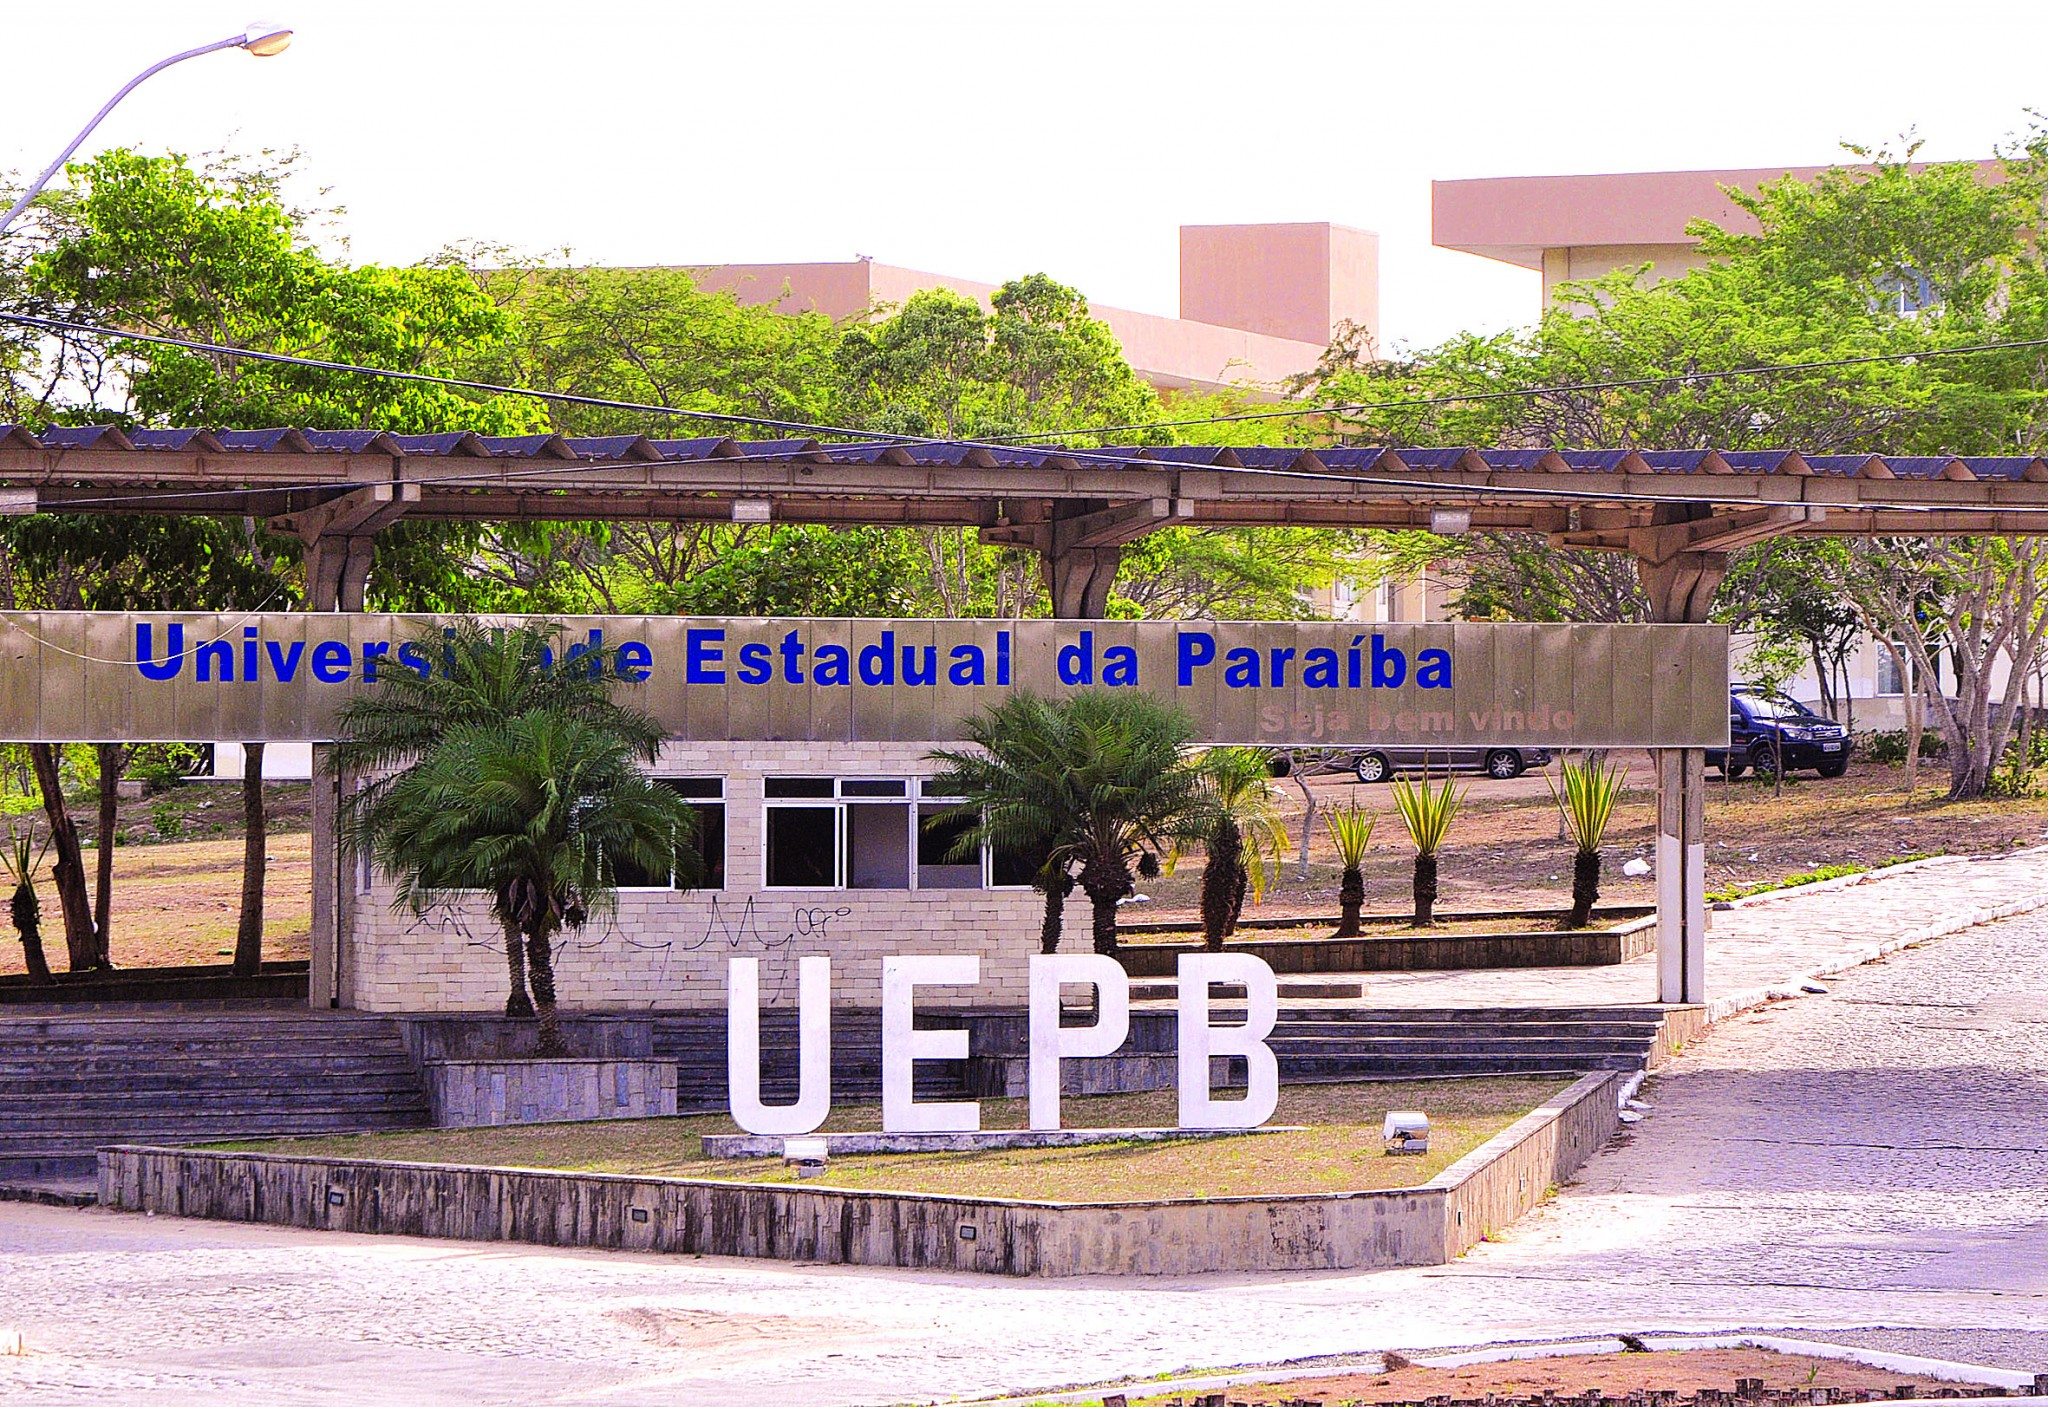
\includegraphics[width=0.8\textwidth]{imagens/entrada-uepb}\\
    {\small Fonte: Autoria própria.}
\end{figure*}

A Figura~\ref{fig:malha} exemplifica a inserção de figuras por meio do ambiente `figure`, incluindo legenda, rótulo (`label`) e referência cruzada no texto utilizando o comando `\verb|\ref{}|`. O comando

\begin{verbatim}
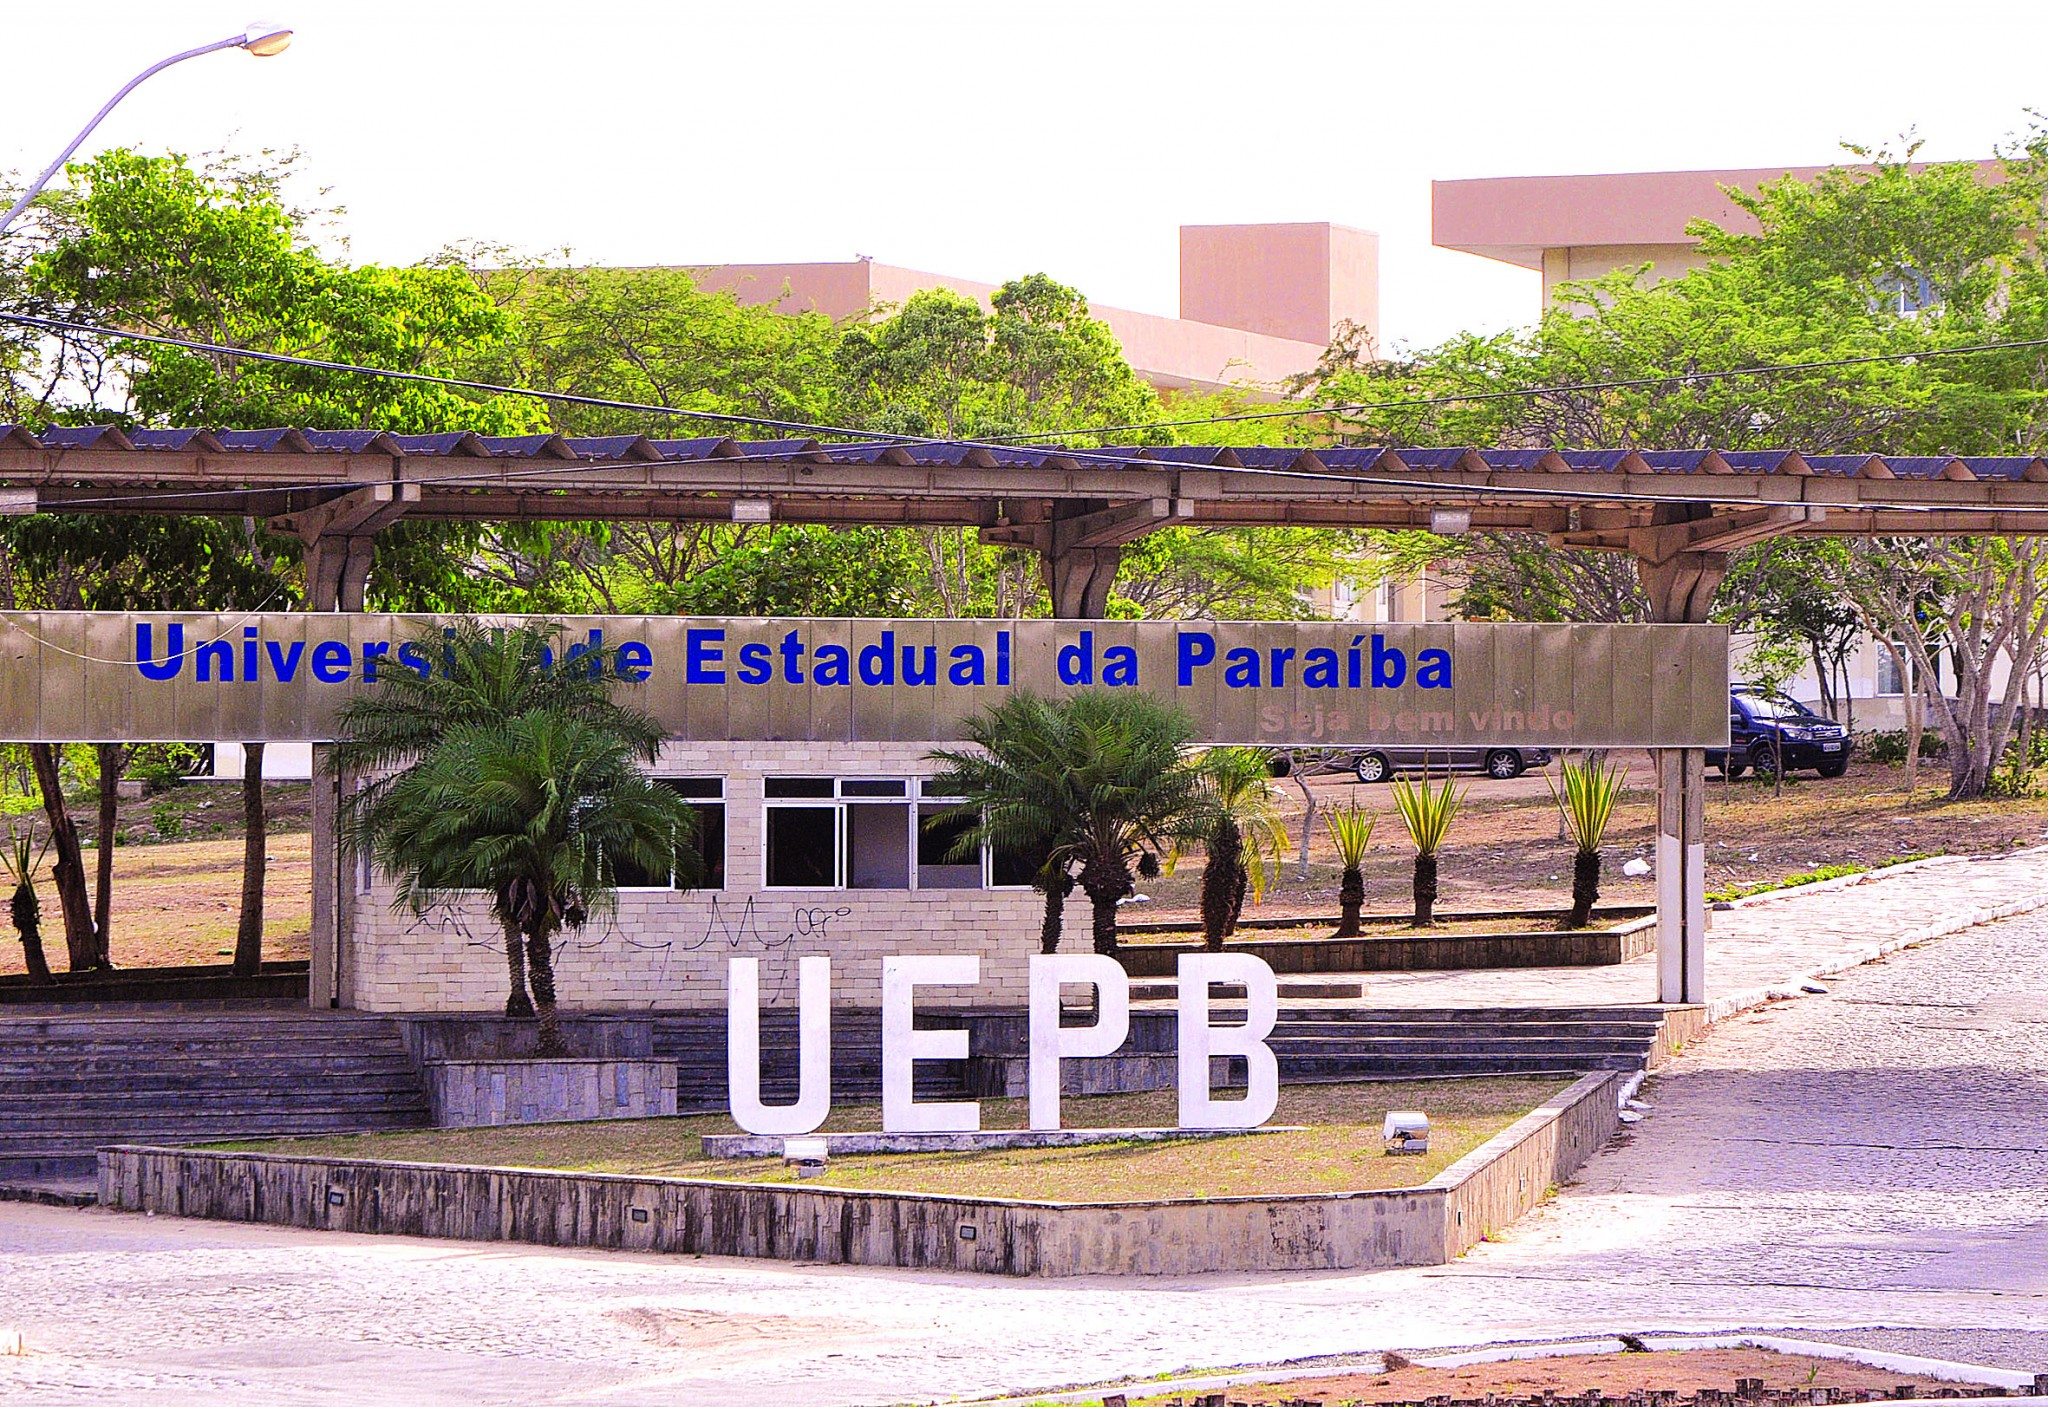
\includegraphics[width=0.8\textwidth]{imagens/entrada-uepb.jpg}
\end{verbatim}

insere a imagem \texttt{entrada-uepb.jpg} localizada na pasta \texttt{imagens}. O argumento opcional

\begin{verbatim}
[width=0.8\textwidth]
\end{verbatim}

controla o tamanho da figura, onde:

\begin{itemize}
    \item \verb|width| especifica que será definida a \textbf{largura} da imagem;
    \item \verb|0.8| indica que a figura ocupará \textbf{80\%} da largura disponível para o texto;
    \item \verb|\textwidth| representa a largura da área útil do texto da página, excluindo as margens.
\end{itemize}

Dessa forma, a imagem é redimensionada automaticamente, preservando sua proporção original.

Alguns exemplos de utilização são apresentados a seguir:

\begin{verbatim}
\includegraphics[width=0.5\textwidth]{figura}
\end{verbatim}

A figura ocupará 50\% da largura do texto.

\begin{verbatim}
\includegraphics[width=\textwidth]{figura}
\end{verbatim}

A figura ocupará toda a largura disponível do texto.

\begin{verbatim}
\includegraphics[width=6cm]{figura}
\end{verbatim}

A figura terá largura fixa de 6 cm.

Também é possível definir a altura da imagem utilizando o parâmetro \verb|height| ou combinar diferentes opções de redimensionamento conforme a necessidade do documento.

O exemplo seguinte ilustra a formatação de uma \textbf{citação direta longa}, conforme recomendado pela ABNT, utilizando recuo de 4 cm, fonte 10 pt e espaçamento simples.

\begin{adjustwidth}{4cm}{0cm} 
\small \singlespacing 
Este é apenas um texto ilustrativo para demonstrar a formatação de uma citação direta longa. Substitua-o pelo trecho original a ser citado, incluindo a referência bibliográfica correspondente e, quando aplicável, a indicação da página.
\end{adjustwidth}

Os demais capítulos deste template apresentam exemplos semelhantes para tabelas, equações, algoritmos, listas, referências bibliográficas e demais elementos frequentemente utilizados na elaboração de trabalhos acadêmicos em conformidade com as normas da ABNT.

Ao redigir o seu trabalho acadêmico, é fundamental manter o padrão na apresentação de termos técnicos. Por exemplo, ao introduzir a \sigla{UEPB}{Universidade Estadual da Paraíba} no texto pela primeira vez, o comando se encarregará de imprimir aqui no parágrafo e também na página LISTA DE ABREVIATURAS E SIGLAS o termo completo seguido da sigla entre parênteses. O mesmo comportamento automático ocorrerá ao mencionarmos a \sigla{UFPB}{Universidade Federal da Paraíba} ou a \sigla{ABNT}{Associação Brasileira de Normas Técnicas}. Para utilizar essa funcionalidade no decorrer dos seus parágrafos, você não precisa digitar tudo manualmente; basta utilizar o comando diretamente no código-fonte, escrevendo \verb|\sigla{SIGLA}{Significado Completo da Sigla}|. Outros exemplos:

\begin{verbatim}
\sigla{UEPB}{Universidade Estadual da Paraíba}
\sigla{UFPB}{Universidade Federal da Paraíba}
\sigla{UFCG}{Universidade Federal de Campina Grande}
\sigla{IFPB}{Instituto Federal da Paraíba}
\sigla{USP}{Universidade de São Paulo}
\sigla{UNICAMP}{Universidade Estadual de Campinas}
\sigla{UFRJ}{Universidade Federal do Rio de Janeiro}
\sigla{UFMG}{Universidade Federal de Minas Gerais}
\end{verbatim}

%----------
%--- RESULTADOS

\chapter{FUNDAMENTAÇÃO TEÓRICA}
\thispagestyle{myheadings}

Este capítulo apresenta o embasamento teórico que fundamenta esta pesquisa, abordando os 
conceitos essenciais de Big Data e de integração de dados via ETL 
(\textit{Extract, Transform, Load}). Inicialmente, exploram-se a evolução do paradigma de 
Big Data, suas dimensões fundamentais (os 5 Vs) e os elementos de sua arquitetura. 
Em seguida, detalham-se as etapas e aplicações dos processos de ETL, suas variações 
(como o paradigma ELT), as principais ferramentas utilizadas pelo mercado e os aspectos 
decisivos para o projeto de pipelines eficientes de dados.

\section{Big Data}

Embora não exista uma definição única e consensual para Big Data, observa-se um certo 
consenso sobre as características que definem o Big Data. Para a Oracle, Big Data são 
dados que contêm maior variedade, chegando em volumes crescentes e com mais velocidade 
\cite{oracle_bigdata}. Já para o Google, o Big Data é um conjunto de dados maior e mais 
complexo, de modo que software tradicional não consegue processá-los e gerenciá-los 
\cite{googlecloud2025bigdata}.

Com base nessas definições, podemos observar um certo padrão para o Big Data, grande 
variedade, o alto volume e a velocidade com que os dados são gerados. Esses elementos 
convergem para uma das abordagens mais difundidas na literatura, os 3 Vs, proposto por 
Doug Laney. Nesse contexto, o Big Data é caracterizado por três dimensões fundamentais: 
volume, velocidade e variedade \cite{laney2001}.

No que se refere ao volume, este diz respeito à gigantesca quantidade dos dados gerados e 
armazenados, 90\% dos dados existentes no mundo hoje foram criados somente nos últimos dois 
anos \cite{sherman2015business}. Essa crescente no volume de dados gerados deve-se principalmente a 
fatores como a digitalização das atividades humanas, a popularização da internet e aumento 
da capacidade de armazenamento de dados.

Em relação a velocidade, ela está relacionada com a rapidez com que os dados são produzidos 
junto a necessidade de processá-los em tempo real. Atualmente dependemos da velocidade de 
alguns desses dados. "É extremamente útil receber uma notificação imediata do banco quando 
uma transação fraudulenta é detectada […]" \cite[p. 26]{sherman2015business}.

Quanto à variedade, essa característica refere-se à diversidade de fontes de origem dos dados, 
bem como aos diferentes formatos em que eles podem ser representados, como imagens, áudios, textos 
e vídeos, além de dados semiestruturados, a exemplo de documentos XML (\textit{eXtensible Markup Language}) 
e JSON (\textit{JavaScript Object Notation}). Nesse contexto, "atualmente, as empresas podem coletar 
dados de publicações em redes sociais sobre seus produtos […] assim como lidar com dados 
valiosos gerados em planilhas e documentos de texto" \cite[p. 27]{sherman2015business}.

Ademais, a definição de Big Data em termos dos 3 Vs evoluiu, ganhando dois Vs adicionais 
de veracidade e valor, formando os 5 Vs do Big Data. A veracidade, se refere à confiabilidade
e à qualidade dos dados, considerando aspectos como inconsistências, ruídos e possíveis 
incertezas presentes nas informações. Já o valor diz respeito à capacidade de extrair 
insights úteis e relevantes a partir dos dados, transformando-os em informação estratégica 
que possa apoiar a tomada de decisão e gerar benefícios para as organizações.

No mais, as características intrínsecas representadas pelos Vs do Big Data permitem 
diferenciá-lo dos modelos tradicionais de dados. Estes, por sua vez, são geralmente 
limitados a volumes menores, como gigabytes, o que torna seu armazenamento e processamento 
mais viáveis \cite{siddiqui2024bigdata}. Além disso, as fontes de dados tradicionais tendem a ser 
mais estruturadas e centralizadas, incluindo bases operacionais, registros de transações e 
sistemas de planejamento de recursos empresariais \cite{siddiqui2024bigdata}.

Diante das limitações dos modelos tradicionais de dados, incapazes de lidar com as demandas 
do Big Data, novas ferramentas e paradigmas surgiram a fim de resolver esses problemas. 
Modelos de programação como o MapReduce permitiram a organizações como a Apache 
desenvolverem todo um ecossistema voltado para solução de problemas envolvendo o Big Data, 
hoje ferramentas como o Apache Hadoop são amplamente utilizadas em empresas convencionais 
\cite{white2012hadoop}.

Desse modo, o Big Data configura-se como um paradigma caracterizado pelos 5 Vs, superando as limitações 
dos modelos tradicionais de processamento de dados. Nesse contexto, a adoção de tecnologias, como aquelas 
pertencentes ao ecossistema Apache, evidencia a necessidade de novas abordagens para o tratamento de grandes 
volumes de dados. Assim, torna-se relevante compreender o contexto de evolução dessas tecnologias e suas 
aplicações em ambientes de Big Data.

\subsection{Contextualização do Big Data}

O cenário de Big Data surgiu naturalmente como resposta ao acelerado processo de digitalização
das atividades humanas que se intensificou no início dos anos 2000. Embora, segundo 
\citeonline{gandomi2015beyond}, o conceito de Big Data provavelmente teve origem em conversas informais 
durante almoços na Silicon Graphics Inc. (SGI) em meados da década de 1990.

A partir dessas primeiras décadas, o Big Data passou a evoluir à medida que o volume, a 
velocidade e a variedade dos dados se ampliaram. Com esse crescimento, as ferramentas 
tradicionais tornaram-se insuficientes para lidar com esse novo paradigma, o que impulsionou 
o surgimento de novas soluções tecnológicas. Nesse contexto, empresas como Google e 
Microsoft, bem como a Fundação Apache, destacaram-se como importantes provedoras de 
plataformas e soluções para o cenário de Big Data \cite{khamaru2022dynamics}.

Essas novas soluções, se mostraram essenciais para o novo cenário global. Instituições que 
já dependiam de dados viram-se cada vez mais inundadas pelos grandes contingentes de 
informações. Em contrapartida, muitas empresas passaram a enxergar no cenário de Big Data 
uma oportunidade de extrair insights relevantes dos dados, com o objetivo de apoiar a tomada 
de decisões estratégicas, e assim, obter vantagens competitivas.

Nesse sentido, o Big Data passou a atuar de forma integrada às práticas de Business 
Intelligence (BI), ampliando a capacidade analítica e o uso estratégico das informações 
nas organizações. Sob essa ótica, \citeonline{narulita2025bigdata} concluem que o Big 
Data e o Business Intelligence constituem pilares estratégicos na contabilidade gerencial, 
permitindo às organizações obter vantagem competitiva por meio de decisões mais rápidas e 
precisas baseadas em dados.

\subsection{Arquitetura do Big Data}

Uma arquitetura de Big Data gerencia a ingestão, o processamento e a análise de dados muito 
grandes ou complexos para sistemas de banco de dados tradicionais \cite{microsoft2025bigdata}. 
Nesse contexto, a arquitetura organiza-se por meio de diferentes elementos e processos que, 
de forma integrada, viabilizam o tratamento eficiente dos dados ao longo de seu ciclo de vida.

\subsection{Elementos do Big Data}

A infraestrutura de armazenamento é um dos principais pilares do Big Data, é nela que o 
volume massivo e diverso dos dados é armazenado. Dado as características do Big Data, os 
principais mecanismos de armazenamento adotados são os sistemas de arquivos distribuídos, 
NoSQL, NewSQL e outros sistemas de gerenciamento de dados \cite{wang2020architecture}. 

No mais, não basta apenas armazenar dados, sendo necessário processar grandes volumes a 
fim de extrair informações relevantes. Segundo \citeonline{albarznji2022big}, o processamento de Big Data 
é essencial para transformar dados em informação útil, classificando os frameworks em cinco 
categorias principais: \textit{batch processing, streaming processing, real-time processing, 
interactive processing e hybrid processing.}

Nesse contexto, temos que o \textit{batch processing} processa grandes volumes de dados acumulados, 
enquanto o \textit{streaming processing} atua sobre fluxos contínuos de dados. 
Ja o \textit{real-time processing} prioriza respostas com baixa latência, ao passo que o 
\textit{interactive processing} permite consultas \textit{ad-hoc} (consultas formuladas sob demanda) 
e exploração dinâmica dos dados. Por fim, o \textit{hybrid processing} combina duas ou mais dessas 
abordagens para atender a diferentes demandas operacionais e analíticas.

Ademais, os dados devem ser coletados a partir de uma ou mais fontes. Nesse contexto, os 
sistemas de ingestão de dados são responsáveis pela coleta e integração dessas informações. 
Assim, ferramentas de ETL são amplamente utilizadas nesse processo, permitindo a extração, 
transformação e carregamento de diferentes tipos de dados \cite{wang2020architecture}.

Por fim, as ferramentas de Business Intelligence permitem que os usuários interajam com 
a infraestrutura de dados por meio de recursos como visualização, consultas, dashboards 
e análises preditivas \cite{sherman2015business}. Essas ferramentas são essenciais para a extração 
de insights relevantes a partir dos dados. Elas são o destino final no que tange a 
utilidade dos dados.

\subsection{Processos do Big Data}

Os processos da arquitetura de dados abrangem a preparação dos dados, o data 
franchising, as atividades de Business Intelligence (BI), bem como o gerenciamento 
de dados e de metadados. A preparação envolve atividades como coleta, transformação, 
limpeza e armazenamento. Já o data franchising refere-se à reorganização dos dados para fins analíticos. 
Por sua vez, as soluções de BI possibilitam o acesso e a análise desses dados por meio de 
ferramentas específicas. Além disso, o gerenciamento de dados e de metadados estabelece 
padrões, governança e controle sobre os ativos informacionais da organização 
\cite{sherman2015business}.

\section{ETL}

No âmbito dos processos de integração de dados, o ETL (Extract, Transform, Load) 
desempenha papel fundamental no cenário de Big Data. Segundo \citeonline{singh2022etl}, "os 
processos de ETL podem consumir até 80\% do esforço em projetos de BI [...] envolvendo a 
extração de dados de fontes externas, sua transformação para atender às necessidades de 
negócios e, por fim, seu armazenamento em um repositório de informações".

Nesse contexto, a sigla ETL refere-se às etapas de extração (Extract), transformação 
(Transform) e carregamento (Load), que, se executadas de forma estruturada, garantem a 
qualidade, consistência e integridade dos dados. Assim, para uma melhor compreensão de 
sua aplicação, torna-se necessário detalhar cada uma dessas etapas, evidenciando suas 
características, técnicas e desafios no processo de integração de dados.

A primeira etapa do processo de ETL é denominada Extract. Seu principal objetivo consiste
em capturar os dados de interesse a partir de diferentes fontes de dados 
\cite{assisvilela2021realtime}. Nessa fase, realiza-se a identificação, seleção e 
coleta dos dados provenientes de das mais diversas fontes, como bancos de dados 
relacionais, arquivos XML e aplicações externas, Essa etapa garante  que as informações 
relevantes sejam disponibilizadas para as etapas subsequentes.

Após a etapa de extração, os dados passam por um processo de transformação antes de 
serem carregados no destino final. Essa etapa é necessária devido à heterogeneidade 
das fontes e dos formatos de origem. Na fase de Transform, os dados são transformados 
ara corresponder ao esquema de dados de destino, geralmente um data warehouse 
\cite{venkateswarlu2023cloud}.

Por fim, os dados extraídos e transformados precisam ser carregados no repositório de 
destino para que possam ser efetivamente utilizados. Essa etapa, denominada Load, 
consiste na inserção dos dados no banco de dados final \cite{singh2022etl}. Trata-se da 
última fase do processo de ETL, sendo responsável por disponibilizar as informações 
de forma estruturada para diversas atividades no cenário de Big Data e BI.

\subsection{Aplicações do ETL}

Os processos de ETL apresentam ampla aplicabilidade nos mais diversos contextos, 
sendo essenciais para a integração, organização e disponibilização de informações em 
diferentes cenários. Dentre as principais aplicações do ETL, destacam-se a integração 
de dados provenientes de múltiplas fontes, processos de limpeza e qualidade de dados, 
a migração de dados e a replicação de dados.

No mais, \citeonline{arsyad2021dynamic} define a integração de dados de múltiplas fontes no contexto de 
ETL como a combinação de técnicas de engenharia e de BI usadas para combinar dados de 
diferentes fontes em informações significativas e valiosas.

Ademais, outra atividade na qual processos de ETL são comumente empregados é no data 
warehousing. O data warehouse é um banco de dados em que dados de várias origens são 
combinados para que possam ser analisados coletivamente. O ETL é geralmente usado para 
mover os dados para um data warehouse \cite{googlecloudetl}.

Outra atividade que se beneficia das etapas de um ETL, principalmente no que diz respeito
a etapa de Transform, é a limpeza e qualidade de dados. A limpeza de dados remove erros 
e mapeia os dados de origem para o formato de dados de destino
\cite{aws2026etl}.

Ademais, as ferramentas de ETL são amplamente utilizadas para migração de dados e 
para a replicação de bancos de dados. Segundo \citeonline{googlecloudetl}, as 
empresas estão movendo seus dados e aplicativos locais para a nuvem, a fim de 
economizar dinheiro, nesse contexto, o ETL é muito usado para executar essas 
migrações. No mais, a \citeonline{ibm2026etl} reforça que, o processo de data replication 
(Replicação de Dados) é frequentemente listada como um método de integração de dados que envolve ETL.

\subsection{Variações ETL e ELT}

O modelo de ETL é o mais tradicional e mais utilizado no Big Data; entretanto, não é o único. 
Existem outras variações do processo, como o ELT (\textit{Extract, Load, Transform}). 
Embora ETL e ELT sejam métodos de integração de dados, a diferença entre eles está no momento da 
transformação de dados. O ETL processa os dados transformando-os antes de carregá-los no sistema de 
destino. No ELT, os dados são carregados no sistema de destino no formato bruto e depois transformados 
\cite{googlecloudetl}.

Ademais, o modelo ELT mostra-se especialmente vantajoso em ambientes de destino com alta 
capacidade de processamento ou quando há necessidade de maior flexibilidade analítica. 
Nesse contexto, \citeonline{naphade2025evolution} destaca que o paradigma ELT aproveita o processamento massivamente
paralelo das plataformas modernas, transferindo a lógica de transformação para o ambiente de 
destino. Tal abordagem é particularmente relevante em cenários cujos requisitos analíticos 
estão em constante evolução.

\subsection{Ferramentas de ETL}

Dado o amplo uso do ETL e de seus derivados, é natural que empresas e instituições tenham 
desenvolvido ferramentas e frameworks voltados para esse tipo de processo. Nesse contexto, 
destacam-se soluções como o Apache Airflow, o SQL Server Integration Services (SSIS), o 
Apache NiFi e o Pentaho Data Integration, amplamente utilizadas na construção e gerenciamento 
de pipelines de dados.

\begin{itemize}
    \item \textbf{Apache Airflow:} é uma ferramenta de código aberto voltada à automação de fluxos de 
    trabalho. o Airflow surgiu como alternativa às ferramentas tradicionais de ETL e sendo 
    projetado para orquestrar processos computacionais complexos de forma dinâmica e escalável 
    \cite{eeti2022efficient}. Além disso, sua flexibilidade permite a integração com ferramentas de 
    processamento distribuído, como o Apache Spark. No mais, a plataforma baseia-se no conceito 
    de grafos acíclicos direcionados (DAGs) e utiliza a linguagem Python para a programação dos 
    fluxos. 

    \item \textbf{SSIS:} o SQL Server Integration Services (SSIS) é uma plataforma da Microsoft 
    voltada à integração e transformação de dados, amplamente utilizada na construção de processos de ETL. 
    Segundo \citeonline{microsoftssis}, o SSIS é utilizado para resolver problemas de negócios 
    complexos. Ademais, o SSIS se destaca como uma plataforma poderosa para executar processos 
    de ETL, permitindo que as empresas manipulem grandes volumes de dados, garantindo precisão e 
    consistência \cite{banoth2024ssis}.

    \item \textbf{Apache NIFI:} é uma ferramenta ETL de código aberto usada para automatizar fluxos que 
    lidam com dados em tempo real. O NiFi foi desenvolvido pela Apache Software Foundation e é 
    adequado para tarefas de fluxo de dados, processamento e interação com sistemas, tudo isso 
    apresentado por meio de um sofisticado fluxograma gráfico \cite{singu2022automation}. 

    \item \textbf{Pentaho:} é uma plataforma de Business Intelligence amplamente utilizada para 
    integração, transformação e análise de dados. A ferramenta possibilita a execução de 
    processos de ETL, além de oferecer suporte à criação de relatórios, dashboards e outros 
    mecanismos de visualização. Segundo \citeonline{demussa2018business}, o Pentaho dispõe de uma 
    infraestrutura completa para a realização de operações de BI, abrangendo desde ferramentas 
    de ETL até mecanismos de acesso, controle e suporte à elaboração de relatórios e painéis 
    analíticos.
\end{itemize}

\subsection{Projeto de ETL}

O projeto de um ETL consiste na definição de estratégias e técnicas para a coleta, 
tratamento e disponibilização de dados provenientes de múltiplas fontes. Essa etapa é 
fundamental, pois garante que os dados sejam integrados, consistentes e adequados para 
análises. Um projeto de ETL bem estruturado deve considerar aspectos como qualidade dos dados, 
desempenho, escalabilidade e governança, assegurando que as informações estejam disponíveis de 
forma confiável para apoio à tomada de decisão.

\begin{itemize}
    \item \textbf{Data Extraction:} a etapa de extração de dados (Data Extraction) é responsável por 
    coletar dados de diferentes fontes, como bancos de dados relacionais, arquivos, APIs e 
    sistemas, planilhas etc. Essa fase é crítica, pois impacta diretamente a qualidade e a 
    integridade das etapas subsequentes do processo de ETL. A extração pode ocorrer de forma 
    completa ou incremental, sendo esta última utilizada para capturar apenas dados novos ou 
    modificados, reduzindo o volume de processamento e aumentando a eficiência do sistema. 
    Além disso, é importante que o processo de extração minimize impactos nos sistemas de 
    origem, garantindo a continuidade das operações.

    \item \textbf{Data Franchising:} o data franchising refere-se ao processo de disponibilização dos 
    dados já tratados em repositórios voltados ao consumo pelos usuários. Essa abordagem 
    consiste em empacotar os dados em estruturas como data marts (subconjuntos de dados 
    orientados a áreas específicas) ou cubos analíticos, facilitando o acesso, a compreensão 
    e a utilização das informações por analistas e gestores. Embora essa prática gera 
    redundância em relação ao data warehouse, trata-se de uma redundância controlada e 
    intencional, que visa melhorar o desempenho e a usabilidade dos dados. Ademais, o data 
    franchising ocorre após as etapas de preparação e transformação, garantindo que apenas 
    dados consistentes e estruturados sejam disponibilizados \cite{sherman2015business}.

\end{itemize}















%----------
%--- METODOLOGIA

\chapter{METODOLOGIA}
\thispagestyle{myheadings}

Este capítulo apresenta os procedimentos metodológicos adotados no desenvolvimento desta pesquisa.

\section{Classificação da pesquisa}

Esta pesquisa classifica-se como aplicada, pois tem como objetivo gerar 
conhecimentos voltados à solução de um problema prático e específico no contexto da 
SEFAZ-PB. Nesse sentido, foi desenvolvido um novo sistema de ETL para o projeto BDMalhas, 
fundamentado em uma nova arquitetura baseada em tecnologias modernas do ecossistema de Big Data, 
com o objetivo de superar as limitações de desempenho e escalabilidade da solução legada.

Em relação aos objetivos da pesquisa, podemos a caracteriza-la como descritiva e exploratória. 
Seu caráter descritivo se deve pela comparação entre a solução desenvolvida e a solução legada, 
com base em métricas de desempenho, manutenibilidade e utilização de espaço em disco obtidas 
durante os experimentos. Já o caráter exploratório está relacionado à investigação da aplicação 
de uma nova arquitetura para a reestruturação dos processos de ETL na SEFAZ-PB, 
buscando compreender seus benefícios e limitações.

Quanto ao método da pesquisa, adota-se o método hipotético-dedutivo, com abordagem quantitativa. 
Uma vez que parte-se da hipótese de que a reestruturação da arquitetura resultará em melhorias 
significativas de desempenho, escalabilidade e manutenibilidade. Por sua vez, a pesquisa 
caracteriza-se como quantitativa por fundamentar-se na coleta e análise de dados numéricos 
obtidos durante os experimentos, tais como tempos de execução, métricas de manutenibilidade e 
utilização de espaço em disco.

Por fim, a pesquisa é conduzida por meio de um estudo de caso, tomando como objeto de estudo 
o projeto BDMalhas, desenvolvido pelo NUTES em parceria com a SEFAZ-PB. Essa classificação 
decorre do fato de que a pesquisa busca avaliar os efeitos da reestruturação dos processos 
de ETL em um contexto real e específico.

\section{A concretização da solução}

Após o levantamento da arquitetura existente e a identificação de suas limitações, iniciou-se o 
desenvolvimento da nova solução de ETL proposta neste trabalho.

Para isso, definiu-se uma nova arquitetura baseada em tecnologias do ecossistema de Big Data, 
adotando o Apache Airflow como ferramenta responsável pela orquestração dos processos de ETL, o Apache 
Spark como mecanismo de processamento distribuído, um Data Lake em PostgreSQL como fonte dos dados e o 
ClickHouse como banco de dados analítico para a persistência das informações processadas.

Com a arquitetura definida, iniciou-se à implementação dos pipelines de ETL para o projeto BDMalhas. 
Durante essa etapa, buscou-se estruturar os pipelines de forma modular, favorecendo a reutilização 
de componentes e facilitando sua manutenção e evolução.

\section{Procedimentos experimentais e análise}

Após a implementação dos novos pipilines de ETL pra o BDmalhas, foram coletadas métricas como o número de 
nós, a quantidade de dependências entre tarefas e a profundidade dos fluxos, com o objetivo de comparar a 
complexidade estrutural e a manutenibilidade de ambas as arquiteturas.

Essa coleta foi realizada por meio da contagem individual dos elementos presentes nos fluxos correspondentes
a cada um dos quatro documentos fiscais processados pelo BDMalhas, tanto na solução baseada em SSIS quanto 
na arquitetura proposta baseada em Apache Airflow.

Após isso foram realizados experimentos com os quatro tipos de documentos 
fiscais processados pelo BDMalhas: NFe, NFCe, CTe e EFD. Para cada documento, foram executadas 
cargas referentes aos períodos de sete dias, um mês e três meses, compreendidos entre 
janeiro e março de 2020, comparando o desempenho da arquitetura proposta com a solução legada 
baseada em SSIS.

Por fim, foram coletadas métricas referentes ao tempo de execução das cargas, à quantidade de 
registros processados em cada experimento e ao tamanho final das bases analíticas. Os resultados
obtidos foram organizados em tabelas e gráficos, possibilitando a comparação do desempenho da 
arquitetura proposta em relação à solução legada baseada em SSIS.
\chapter{DESENVOLVIMENTO DA SOLUÇÃO}
\thispagestyle{myheadings}

Os resultados e discussões apresentados a seguir referem-se aos experimentos realizados durante 
a reestruturação dos processos de ETL do BDMalhas. As análises baseiam-se nas métricas definidas 
na metodologia, permitindo comparar o desempenho da arquitetura proposta com a solução legada 
baseada em SSIS.

\section{Arquitetura proposta para a reestruturação da plataforma de dados}

A seguir, apresenta-se o sistema de ETL desenvolvido para materializar a proposta de 
reestruturação da plataforma de dados da SEFAZ-PB, utilizando como referência o sistema BDMalhas.
A solução contempla tanto a reestruturação das pipelines de ETL quanto a adoção 
de uma nova arquitetura visando atender às demandas de processamento e análise de grandes 
volumes de dados. Também são apresentados os principais aspectos da implementação da solução.

\section{Arquitetura do BDMalhas}

O BDMalhas é um projeto composto por sistemas integrados que auxiliam o processo de 
fiscalização tributária da SEFAZ-PB por meio da análise de documentos fiscais, como NFe, 
NFCe e EFD. Nesse cenário, os dados oriundos do Sistema de Administração Tributária e 
Financeira (ATF), que atua como \textit{System of Record} (SOR), ou seja, o sistema considerado fonte 
oficial e autorizada das informações tributárias e financeiras da Secretaria. Essas informações 
são coletadas por meio de um processo de ETL implementado em SSIS, e em seguida, armazenados 
em uma área \textit{staging} (área de preparação dos dados). 

Em seguida, a área de \textit{staging} é utilizada para a geração de bases de dados analíticas no 
formato de malhas fiscais, a serem acessadas pelos auditores para atividades de análise através 
do Sistema de Controle e Análise das Malhas Fiscais (SCAMF).

\begin{figure*}[ht!]
    \centering
    \caption{Visao Geral da Arquitetura Antiga do BDmalhas}\label{fig:arq_ant_bdmalha}
    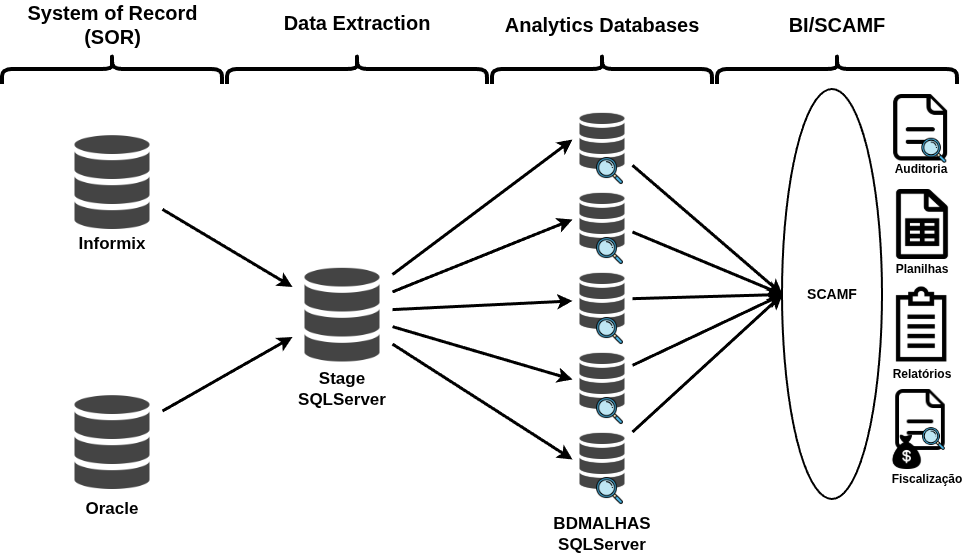
\includegraphics[width=0.8\textwidth]{imagens/ArquiteturaAntiga_bdmalhas}\\
    {\small Fonte: Elaborado pelo autor, 2026}
\end{figure*}

Nesse sentido, a Figura \ref{fig:arq_ant_bdmalha} apresenta a arquitetura de dados do BDMalhas, estruturada nas seguintes 
camadas:

\begin{itemize}
    \item \textbf{System of Record (SOR):} camada responsável pela origem dos dados. Nela encontram-se os 
    bancos de dados transacionais do sistema ATF, implementados nas plataformas Informix e Oracle.

    \item \textbf{Data Extraction:} camada responsável pela extração dos dados. Por meio de processos de 
    ETL (Extract, Transform and Load), os dados são extraídos do SOR, submetidos às transformações 
    necessárias e carregados em uma área intermediária de armazenamento.

    \item \textbf{Analytical Databases:} camada responsável pela consolidação e disponibilização analítica 
    das informações. A partir dos dados armazenados na área de staging, são executados processos 
    de transformação e enriquecimento que resultam na construção de bases analíticas e malhas 
    fiscais destinadas ao consumo pelo SCAMF.

    \item \textbf{BI/SCAMF:} camada de apresentação e consumo das informações. Nessa camada, os dados 
    são disponibilizados aos fiscais e contribuintes por meio do sistema SCAMF, responsável por 
    fornecer recursos de consulta, visualização e análise das informações produzidas pelas camadas 
    anteriores.
\end{itemize}

\section{Arquitetura Reestruturada do BDMalhas}

A nova arquitetura implementada para o BDMalhas incorpora um Data Lake, desenvolvido pela 
Universidade Federal da Paraíba (UFPB) em parceria com a SEFAZ-PB, como principal fonte de 
dados para a etapa de extração. O Data Lake consiste em um repositório centralizado que atua 
no armazenamento e integração de grandes volumes de dados provenientes das diferentes fontes 
da secretaria.

Dessa forma, os processos passam a extrair informações de um ambiente estruturado para cenários 
de Big Data, simplificando as consultas e aumentando a eficiência das etapas de integração e 
processamento dos dados.

Ademais, houve a substituição do SQL Server Integration Services (SSIS) pelo Apache Airflow como 
plataforma de orquestração dos pipelines de dados, juntamente com a adoção do Apache Spark como 
mecanismo de processamento distribuído. Essa mudança  visa proporcionar maior escalabilidade, 
flexibilidade e capacidade de processamento.

Por fim, o banco de dados da camada de staging foi substituído por um banco de dados colunar, 
mais adequado a cenários de Big Data. Esse modelo de armazenamento proporciona maior eficiência 
no processamento de grandes volumes de dados e melhor desempenho em consultas analíticas, 
características essenciais para a nova arquitetura proposta.

\begin{figure*}[ht!]
    \centering
    \caption{Visao Geral da Arquitetura Nova do BDmalhas}\label{fig:arq_nova_bdmalha}
    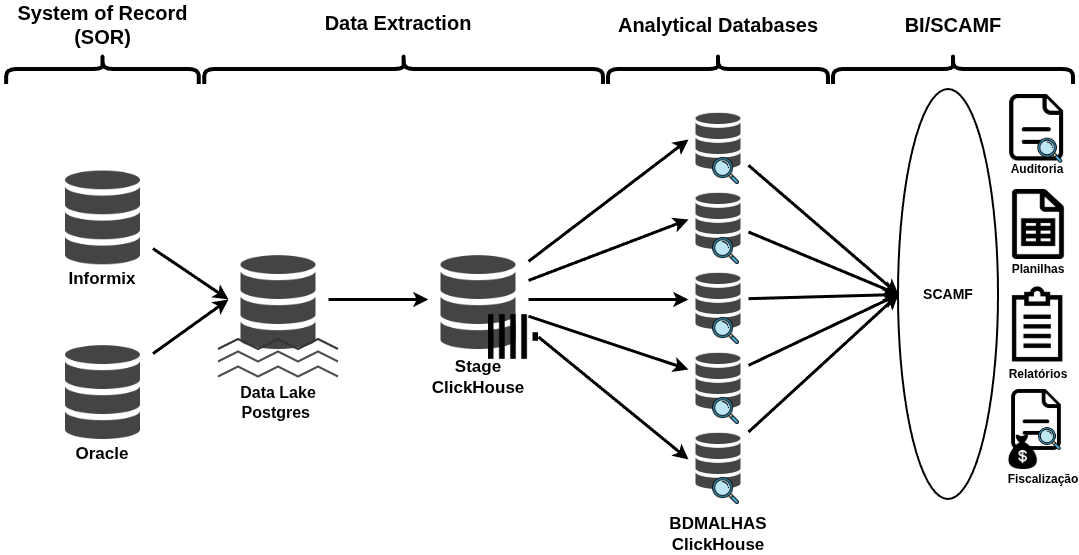
\includegraphics[width=0.8\textwidth]{imagens/ArquiteturaNova_bdmalhas}\\
    {\small Fonte: Elaborado pelo autor, 2026}
\end{figure*}

A Figura \ref{fig:arq_nova_bdmalha} apresenta a nova arquitetura de dados do BDMalhas, com alterações para as 
seguintes camadas:

\begin{itemize}
    \item \textbf{Data Extraction:} passa a ter mais uma camada, um Data Lake implementado em 
    Postgres e gerido pela UFPB, de onde os dados são extraídos, alimentado a base de staging.

    \item \textbf{Analytical Databases:} no \textit{staging}, são executados processos de transformação e 
    enriquecimento que resultam na construção de bases analíticas e malhas fiscais destinadas
    ao consumo pelo SCAMF.
\end{itemize}

Dado o contexto da nova stack tecnológica adotada na reestruturação, o processo de ETL 
inicia-se com a extração dos dados a partir do Data Lake PostgreSQL da SEFAZ-PB. 
O Apache Airflow é responsável pela orquestração dos fluxos de execução, estruturados em 
DAGs (Directed Acyclic Graphs) compostas por tasks executadas de forma sequencial ou 
paralela, mantendo a mesma lógica operacional anteriormente implementada em Microsoft SSIS.

Contudo, diferentemente da arquitetura anterior, o Airflow não realiza diretamente o 
processamento das cargas de dados, atuando apenas como mecanismo de orquestração. 
As operações de transformação e carga de dados são delegadas a um \textit{cluster} Spark composto 
por múltiplos nós computacionais, responsável pelo processamento distribuído dos dados e 
posterior inserção no ambiente de \textit{staging}.

\section{Benefícios e considerações Arquiteturais}

A adoção de Airflow é justificada por proporcionar um ambiente mais flexível e 
desacoplado para construção e manutenção dos pipelines de ETL, permitindo que os 
fluxos sejam desenvolvidos de forma programática, diferentemente da abordagem utilizada 
pelo SSIS. Além disso, a ferramenta disponibiliza aos administradores recursos nativos de 
monitoramento das execuções, rastreamento de falhas e gerenciamento operacional dos 
pipelines, contribuindo para maior controle e confiabilidade do processo.

Junto a isso, destaca-se a adoção do Apache Spark como mecanismo de processamento 
distribuído, com o objetivo de viabilizar o processamento eficiente dos dados em tempo 
hábil, além de permitir escalabilidade horizontal conforme o aumento da demanda 
computacional. Essa abordagem atende diretamente às necessidades dos fiscais, que 
dependem do acesso rápido e confiável às informações processadas para execução de suas 
atividades de fiscalização.

Dessa forma, a combinação entre Airflow e Spark permite construir uma arquitetura mais 
robusta, escalável e aderente às demandas operacionais e estratégicas da secretaria e do 
sistema BDMalhas.

Em síntese, a arquitetura proposta consolida a reestruturação da plataforma de dados do 
BDMalhas por meio da adoção de tecnologias voltadas ao processamento distribuído e à 
orquestração de pipelines, estabelecendo uma base mais escalável e flexível para os 
processos de ETL. Na sequência, é apresentada uma avaliação dos resultados obtidos com essa 
reestruturação, por meio da comparação entre o sistema original e o sistema desenvolvido.
%----------
%--- RESULTADOS

\chapter{RESULTADOS}
\thispagestyle{myheadings}

Esse capítulo busca apresentar e analisar os resultados obtidos a partir da a reestruturação do 
ETL do BDMalhas. Para isso, são comparados indicadores estruturais e de desempenho 
entre o projeto original e a implementação da solução proposta, permitindo assim analisar os ganhos 
alcançados com a solução desenvolvida.

\section{Avaliação da Manutenibilidade da Arquitetura Proposta}

Para avaliar como a reestruturação do ETL do BDMalhas impactou na manutenabilidade do sistema 
foi realizado uma contagem de metricas relacionadas à complexidade estrutural e ao esforço de 
manutenção das implementações original e proposta.

As métricas foram coletadas com base na superfície de design do SSIS, na interface web do Airflow 
e nos arquivos do novo projeto. Para a avaliação, foram considerados o número de nós, a quantidade 
de dependências entre os nós e o número de consultas SQL.


Ademais, a escolha dessas métricas se deu pelo fato de representarem os aspectos 
relacionados à complexidade estrutural e à facilidade de manutenção dos fluxos de ETL. Alem de que,
em conjunto conjunto, elas permitem avaliar o grau de modularização da solução, o nível de 
acoplamento entre as etapas, a complexidade do fluxo de execução e o esforço necessário para 
compreender, modificar e evoluir as pipelines ao longo do tempo.

No mais, as métricas coletadas estão apresentadas na Tabela \ref{tab:comparacao_manutenibilidade}, 
elaborada a partir da contagem dessas medidas em ambas as implementações.


%-------------------
%-----Tabela--------

\begin{table}[htb]
\centering
\caption{Comparação das métricas de manutenibilidade.}
\label{tab:comparacao_manutenibilidade}

\footnotesize
\renewcommand{\arraystretch}{1.2}

\newcolumntype{Y}{>{\centering\arraybackslash}X}

\begin{tabularx}{\textwidth}{|p{4.0cm}|Y|Y|Y|Y|}
\hline
\textbf{Métrica} & \textbf{NFE} & \textbf{NFCE} & \textbf{EFD} & \textbf{CTE} \\
\hline
Nós (SSIS $\rightarrow$ Airflow) &
148 $\rightarrow$ 21 (85,8\%) &
123 $\rightarrow$ 17 (86,2\%) &
222 $\rightarrow$ 76 (65,7\%) &
30 $\rightarrow$ 11 (63,3\%) \\
\hline

Dependências (SSIS $\rightarrow$ Airflow) &
124 $\rightarrow$ 26 (79,0\%) &
108 $\rightarrow$ 13 (88,0\%) &
198 $\rightarrow$ 70 (64,6\%) &
22 $\rightarrow$ 11 (50,0\%) \\
\hline

Consultas SQL (SSIS $\rightarrow$ Airflow) &
102 $\rightarrow$ 9 (91,2\%) &
84 $\rightarrow$ 6 (92,9\%) &
152 $\rightarrow$ 40 (73,7\%) &
30 $\rightarrow$ 6 (80,0\%) \\
\hline

\end{tabularx}

\vspace{0.5em}
{\small Fonte: Elaborado pelo autor, 2026}

\end{table}

A partir da leitura da Tabela \ref{tab:comparacao_manutenibilidade}, ficam evidentes os ganhos de 
manutenabilidade obtidos com a nova solução. Primeiramente, observa-se uma expressiva redução no 
número de nós em todos os quatro fluxos referentes aos diferentes documentos fiscais. Entre eles, 
os fluxos de NFCE e NFE foram os mais beneficiados, apresentando uma redução de aproximadamente 
85\% em relação à implementação original.

Essa expressiva redução deve-se, principalmente, à forma como o projeto original estava estruturado. 
Nos fluxos de NFCE e NFE do SSIS, o processo era dividido em dois grandes blocos de tarefas, 
responsáveis pela extração de notas de emitente e de destinatário. Entretanto, esses blocos eram 
praticamente idênticos, diferenciando-se apenas pelos prefixos "E" e "D" (emitente e destinatário, 
respectivamente) nos nomes das tarefas e por uma cláusula `WHERE` nas consultas SQL, utilizada para 
definir o tipo de nota fiscal a ser processada.

A existência dessa duplicação no projeto original era justificada por limitações do próprio SSIS. 
Em muitos cenários, a ferramenta não conseguia extrair, em uma única execução, todos os dados das 
notas fiscais de emitente e de destinatário devido ao elevado volume de dados. Como consequência, 
a extração frequentemente resultava em erros e perdas de conexão com o banco de dados em razão do 
longo tempo necessário para a execução das consultas.

Desse modo, com a adoção do Apache Spark e a utilização do Data Lake da UFPB como nova fonte de 
dados, optou-se por eliminar a separação entre notas de emitente e de destinatário no novo sistema 
de ETL. Essa mudança permitiu unificar o processamento em um único fluxo, reduzindo, a priori, em 
aproximadamente 50\% tanto o número de nós do workflow quanto o número de consultas SQL necessaras.

Ademais, a utilização do Data Lake e de suas consultas unificadas contribuiu significativamente 
para a redução do número de tarefas do fluxo de ETL. A Figura \ref{fig:fluxo_ssis_mult} apresenta 
um trecho do fluxo da carga de NFe, evidenciando a elevada quantidade de consultas executadas na 
implementação original. Com a adoção do esquema de dados disponibilizado pelo Data Lake, foi possível 
substituir essas múltiplas consultas por uma única consulta ao banco de dados, reduzindo 
significativamente tanto o número de nós da aplicação quanto o de consultas, assim, simplificando o 
pipeline ETL como um todo.

\begin{figure*}[ht!]
    \centering
    \caption{Exemplo de fluxo SSIS que executa multiplas consultas}\label{fig:fluxo_ssis_mult}
    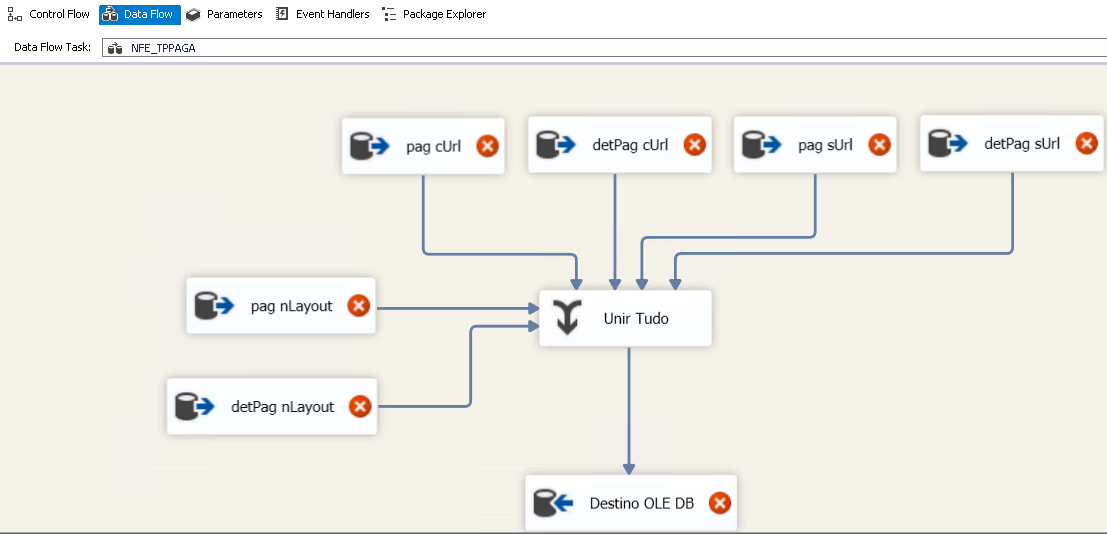
\includegraphics[width=1\textwidth]{imagens/ap_exe_task_com_multiplas_consultas.png}\\
    {\small Fonte: Elaborado pelo autor, 2026}
\end{figure*}

Já os fluxos referentes à EFD e CTE apresentaram uma redução de aproximadamente 64\% no número de 
nós. Embora esse resultado também seja expressivo, ele foi inferior ao observado nos fluxos de 
NFCE e NFE, pois essas cargas não possuíam duplicação de blocos de tarefas destinados ao processamento 
de documentos de emitente e de destinatário na implementação original.

De modo geral, a redução no número de nós desses fluxos foi resultado da junção de tarefas 
responsáveis pelas operações de registro de logs na origem e no destino com as tarefas de
extração e inserção de dados. No projeto SSIS essas tarefas são executadas de forma separada, e 
após análises, optou-se por unifica-las, reduzindo desse modo a complexidade do workflow.

A redução do número de dependecias se deu principalmente pela redução do número de nós do projeto.
Dado que, a eliminação de etapas redundantes diminuíram a quantidade de relações existentes entre as 
tarefas. 

Já as consultas SQL tiveram uma redução drástica quando comparadas ao projeto original. Como já 
mencionado anteriormente, grande parte dessa redução decorre da utilização do Data Lake como fonte 
de dados, eliminando a necessidade da execução de múltiplas consultas. Além disso, a parametrização 
permitiu o reaproveitamento de consultas comuns a diversos trechos do projeto, contribuindo ainda 
mais para a diminuição da quantidade de consultas SQL.

Como resultado, foram obtidas reduções de cerca de 90\% no número de consultas SQL dos projetos 
de NFCE e NFE. Grande parte dessa redução se deve à remoção da estratégia de notas de emitente e 
destinatário. Já os projetos de EFD e CTE também apresentaram reduções expressivas, embora menos 
acentuadas, da ordem de 80\% e 70\%, respectivamente, conforme apresentado na Tabela 
\ref{tab:comparacao_manutenibilidade}.

% Por fim temos que, a reestruturação da arquitetura do ETL promoveu uma redução significativa da 
% complexidade dos pipelines em relação à solução originalmente implementada em SSIS. Essa simplificação 
% foi possível devido à adoção de uma abordagem programática devido ao uso do Apache Airflow 
% como plataforma de orquestração e à reorganização dos dados proporcionada pelo Data Lake, 
% permitindo maior reutilização de código e redução da quantidade de componentes dos workflows.

% Nesse sentido, temos que os ganhos de manutenabilidade decorreram principallmente 
% do reaproveitamento de código SQL, lógica de processamento e regras de negócio. Adicionalmente, a 
% utilização do Data Lake da UFPB e de seu modelo de dados possibilitou a substituição de diversas 
% consultas SQL por uma única consulta, reduzindo a duplicação de codigo SQL e simplificando a
% manutenção da solução como um todo, conforme evidenciado pela Tabela 
% \ref{tab:comparacao_manutenibilidade}.


\section{Análise comparativa de desempenho}

Antes de mais nada, devemos reiterar que a quantidade de workers do Spark influencia diretamente a 
capacidade de processamento paralelo do sistema. No contexto do ambiente avaliado, foi possível
executar até seis tasks simultaneamente, contudo esse paralelismo pode variar conforme o número 
de workers do cluster Spark e as configurações do Airflow.

\begin{grafico}[ht!]
    \centering
    \caption{Tempos de execução das cargas ETL.}\label{graf:tempo_exec}
    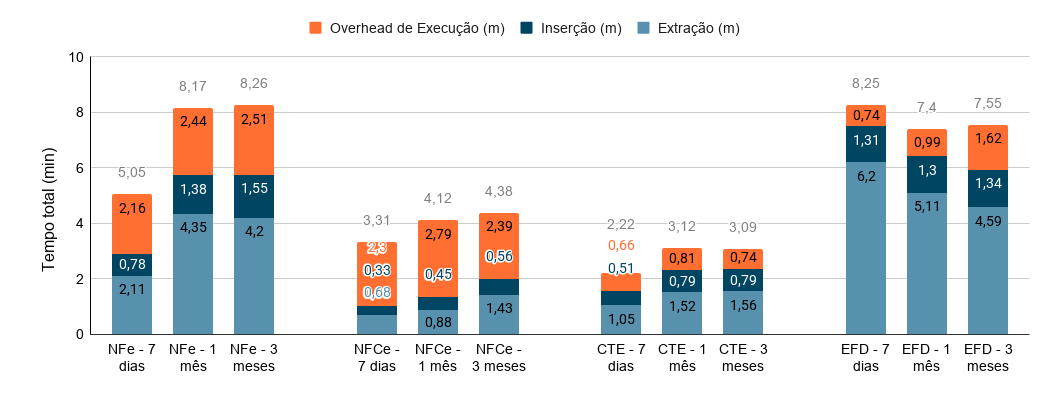
\includegraphics[width=1\textwidth]{imagens/grafico_tempo_exec}\\
    {\small Fonte: Elaborado pelo autor, 2026}
\end{grafico}

No mais, para avaliar o desempenho das cargas, foram executados experimentos 
com os quatro tipos de documentos fiscais em três intervalos temporais distintos: 
7 dias, 1 mês e 3 meses. Em cada execução, foram registrados separadamente os tempos de 
extração, inserção, overhead de execução e o tempo total da execução, permitindo uma 
análise detalhada do comportamento de cada etapa. Os resultados são apresentados 
no Gráfico \ref{graf:tempo_exec}.

Esses resultados foram coletados por meio de funcionalidades da biblioteca \textit{datetime} do 
Python e registrados na tabela \textit{sql\_log\_validacao}, responsável por armazenar os registros 
que permitem o acompanhamento da execução das cargas.

No geral, é perceptível que o novo projeto apresentou um bom tempo de execução, uma vez que nenhuma 
das cargas ultrapassou dez minutos. Contudo, deve-se lembrar que a execução das cargas ocorreu em um 
ambiente experimental, e os dados foram extraídos de uma réplica do Data Lake original. 
Essa réplica contém um volume de dados significativamente menor que o Data Lake original.

A partir do Gráfico \ref{graf:tempo_exec}, observa-se que, na maioria dos cenários avaliados, 
a etapa de extração dos dados foi a que demandou o maior tempo de execução. Em seguida, destaca-se o 
\textit{overhead} introduzido pelo Airflow e pelo Spark, enquanto a etapa de inserção dos dados 
apresentou, de forma consistente, os menores tempos de processamento.

O Gráfico \ref{graf:tempo_exec} tambem deixa perceptivel que a medida que o intervalo de tempo 
aumenta, ocorre um crescimento gradual do tempo de execução. Entretanto, esse crescimento 
mostrou-se aproximadamente proporcional ao volume processado, indicando um comportamento consistente 
da solução para diferentes quantidades de dados.

A única carga que não apresenta esse comportamento de crescimento gradual é a carga de EFD. Sua 
execução para um período de 7 dias resultou em um tempo de execução superior ao observado para os 
períodos de 1 e 3 meses. Isso provavelmente ocorreu devido à pequena quantidade de dados 
extraídos por esse fluxo. A Tabela \ref{tab:desempenho_cargas} evidencia esse comportamento, 
visto que a carga referente ao período de 3 meses extraiu apenas 2.440 registros. Considerando 
esse baixo volume de dados, é esperado que ocorram pequenas discrepâncias nos tempos de execução.

Também deve ser mencionado que a carga de EFD apresentou o maior tempo de extração, mesmo sendo a 
que extraiu a menor quantidade de registros entre todas as cargas. Isso ocorre por ela possuir o 
maior número de tarefas (nós), totalizando 76, conforme evidenciado na Tabela 
\ref{tab:comparacao_manutenibilidade}.

Outra coisa que podemos relatar a partir dos dados é que o tempo de \textit{overhead} se mantém
relativamente constante, variando pouco no contexto dos diferentes intervalos de tempo do mesmo 
documento fiscal. Isso se deve principalmente a como o fluxo dos pipelines dos documentos fiscais
estão organizados, ao número de tasks e ao número de tasks executadas em paralelo. Tanto é que
pipelines semelhantes, como os de NFE e NFCE, apresentam tempos de \textit{overhead}
tambem semelhantes. No mais, essas semelhanças entre NFE e NFCE podem ser observadas ao 
visualizar as Figuras \ref{fig:nfe} e \ref{fig:nfce} presentes no Apêndice~\ref{apend:a}.

Por fim, observa-se que os tempos de inserção permaneceram baixos em todos os fluxos avaliados, 
apresentando pouca variação mesmo com o aumento do período de dados processados. Enquanto o tempo 
de extração tende a crescer conforme o volume de registros, a etapa de inserção manteve-se 
relativamente estável, variando entre aproximadamente 0,33 e 1,55 minutos.

\subsection{Desempenho do projeto original}

\begin{grafico}[ht!]
    \centering
    \caption{Tempos de execução das cargas no projeto original.}\label{graf:tempo_ssis}
    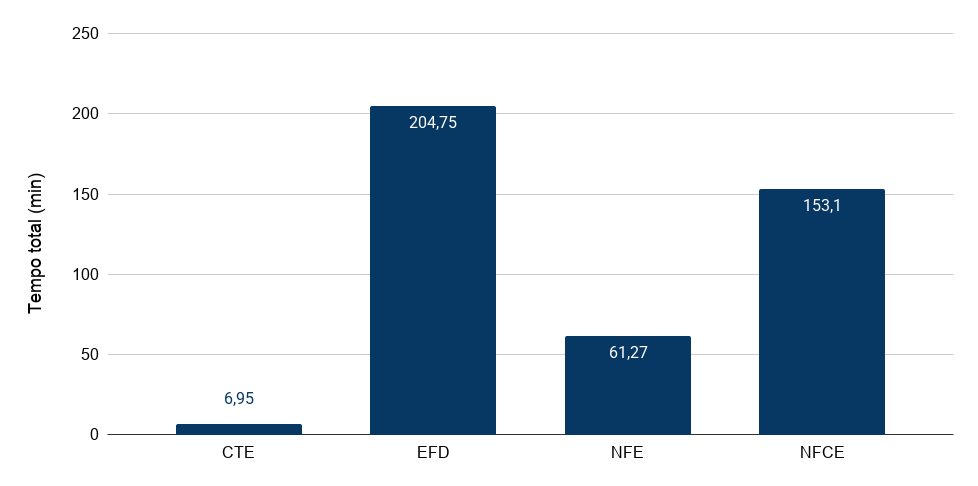
\includegraphics[width=1\textwidth]{imagens/tempos_ssis.png}\\
    {\small Fonte: Elaborado pelo autor, 2026}
\end{grafico}

Foi realizada uma execução do sistema original com o objetivo de obter os tempos de execução de cada
um dos fluxos referentes aos quatro tipos de documentos fiscais. A execução das cargas foi acionada 
pela equipe do Núcleo de Tecnologia Estratégica em Saúde (Nutes), responsável pelo desenvolvimento 
e manutenção do BDMalhas.

Desse modo, devido à dependência da equipe de membros de desenvolvimento para iniciar a execução do 
sistema baseado em SSIS, tornou-se inviável realizar sucessivas execuções das mesmas cargas para 
diferentes períodos de tempo. Por esse motivo, foi executada apenas uma carga correspondente ao 
período de janeiro a março de 2020 (3 messes).

Além disso, como o projeto de ETL original em SSIS não possui mecanismos para obter separadamente 
os tempos de extração, inserção e \textit{overhead}, foi contabilizado apenas o tempo total de 
execução.

O Gráfico \ref{graf:tempo_ssis} apresenta os tempos de execução em minutos para os quatro fluxos
de ETL, obtidos a partir da execução da solução legada no ambiente de produção. No mais, os 
dados presente no gráfico evidenciam grandes variação entre as cargas. 

A carga de CTE registrou o menor tempo de processamento, totalizando 6,95 minutos, seguida pela 
carga de NFE, com 61,27 minutos. Já as cargas de NFCE e EFD demandaram tempos significativamente 
maiores, alcançando 153,10 e 204,75 minutos, respectivamente.

Por fim, observa-se que a carga de EFD foi a que apresentou o maior tempo de execução, ultrapassando
três horas de processamento. Em contrapartida, a carga de CTE foi concluída em menos de sete minutos. 
Essa diferença evidencia que os tempos de execução variam consideravelmente entre os diferentes 
fluxos, dado que cada carga possui características próprias que influenciam diretamente sua 
duração.

\subsection{Limitações da comparação experimental}

Antes de mais nada, é importante destacar algumas limitações na comparação dos tempos de execução 
entre os dois projetos. Primeiramente, deve-se reiterar que ambos os sistemas foram executados em 
ambientes distintos. Portanto, é esperado que os resultados obtidos sejam influenciados pelas 
diferenças de infraestrutura.

Ademais, o projeto original, desenvolvido em SSIS, possui acesso direto às bases de produção do 
sistema ATF, armazenadas nos bancos Oracle e Informix, que contêm terabytes de informações fiscais. 
Em contrapartida, o projeto implementado em Airflow foi executado utilizando uma cópia do Data Lake 
original com um volume de dados significativamente menor.

Além disso, tanto as consultas SQL quanto o esquema de dados das duas versões do Data Lake ainda não
estão em sua plenitude. Em outras palavras, o esquema de dados do Data Lake ainda não representa 
integralmente o que existe nas bases de produção Oracle e Informix. Ainda há tabelas, colunas, campos,
relacionamentos e registros que precisam ser incorporados ou refinados.

Um exemplo disso é a própria carga de EFD. No projeto original, os dados a serem carregados são 
filtrados pela coluna \textit{sqcontrib}, responsável por armazenar o sequencial do contribuinte. 
Entretanto, no contexto da reestruturação, até o momento da redação deste trabalho, essa coluna 
ainda não havia sido incorporada ao Data Lake, tampouco existia um campo equivalente.

Diante desse cenário, para viabilizar a execução da carga de EFD no novo ambiente, utilizou-se a 
coluna de CNPJ do contribuinte como critério de filtragem dos dados em substituição ao 
\textit{sqcontrib}. Contudo, essa abordagem não estabelece uma correspondência exata com a 
implementação original, o que influencia os dados efetivamente carregados e, consequentemente, os 
resultados obtidos.

Ademais, diante desses fatores, é esperado que algumas das consultas disponibilizadas pela UFPB 
ainda não reflitam integralmente o comportamento das consultas implementadas no projeto original 
em SSIS, seja por diferenças no esquema de dados, seja pela ausência de determinados campos ou 
ajustes ainda pendentes. 

Dessa forma, serão necessárias futuras iterações com a equipe da UFPB para refinar o esquema de 
dados e as consultas de extração, a fim de se aproximar cada vez mais do ambiente de produção.

\section{Comparação do Projeto novo x antigo}

Tendo em vista as limitações apresentadas na subsseção anterior, podemos seguir com a 
apresentação dos resultados.

Após a execução das cargas dos quatro tipos de documentos fiscais em ambas as versões do ETL do 
BDMalhas, considerando o período compreendido entre 1º de janeiro e 31 de março de 2020, foram 
obtidos os dados referentes aos tempos de execução e às quantidades de registros extraídos e 
inseridos nos bancos de destino de ambas as aplicações. Esses resultados são apresentados na 
Tabela \ref*{tab:desempenho_cargas}, que relaciona a quantidade de registros processados com o 
tempo total de execução das cargas.


\begin{table}[H]
\centering
\caption{Desempenho das cargas executadas nas implementações avaliadas}
\label{tab:desempenho_cargas}
\begin{tabular}{lrrr}
\toprule
\textbf{Implementação} & \textbf{Registros} & \textbf{Tempo (min)} & \textbf{Registros/min} \\
\midrule
CTE -- SSIS           &    176.749 &   6,95 & 25.431,51 \\
CTE -- Nova solução   &    113.049 &   3,09 & 36.585,44 \\
\addlinespace
EFD -- SSIS           & 16.895.738 & 204,75 & 82.518,87 \\
EFD -- Nova solução   &      2.440 &   7,55 &    323,18 \\
\addlinespace
NFCE -- SSIS          &  4.253.188 & 153,10 & 27.780,46 \\
NFCE -- Nova solução  &     36.793 &   4,38 &  8.400,23 \\
\addlinespace
NFE -- SSIS           &  1.000.420 &  61,27 & 16.328,06 \\
NFE -- Nova solução   &    651.385 &   8,25 & 78.955,76 \\
\bottomrule
\end{tabular}

\caption*{\small Fonte: Elaborado pelo autor, 2026}
\end{table}

A princípio, é evidente que a quantidade de registros obtida para os mesmos documentos fiscais não 
é a mesma entre as duas implementações. Nos casos da EFD e da NFCE, as diferenças são bastante 
expressivas, chegando à ordem de milhões de registros. Isso se deve, principalmente, à utilização 
da réplica do Data Lake, que possui um volume de dados significativamente menor que o ambiente 
original.

No caso da carga de CTE, a nova solução reduziu o tempo de execução de 6,95 para 3,09 minutos, 
representando uma diminuição de 55,54\% no tempo de execução. 
Embora que, a nova solução tenha processado uma quantidade menor de registros. Contudo sua taxa 
média de processamento foi superior, passando de 25.431,51 para 36.585,44 registros por minuto, 
o que representa um aumento de 43,86\% em relação à solução baseada em SSIS.

Para a carga de EFD, a nova solução executou a carga em apenas 7,55 minutos, frente aos 204,75 
minutos da implementação em SSIS. Entretanto, essa comparação deve ser interpretada com cautela, 
pois a nova solução processou apenas 2.440 registros, enquanto a versão original carregou 16.895.738 
registros.

Na carga de NFCE, a nova solução concluiu a execução em 4,38 minutos, contra 153,10 minutos da 
implementação em SSIS. Contudo, assim como no caso da EFD, houve uma diferença significativa na 
quantidade de registros processados, impossibilitando uma comparação direta da taxa de processamento 
entre as duas implementações.

Por fim, na carga de NFE, a nova solução reduziu o tempo de execução de 61,27 para 8,25 minutos, 
correspondendo a uma redução de 86.54\% no tempo de execução. Mesmo processando uma quantidade 
menor de registros, essa carga apresentou um desempenho bem superior, atingindo
78.955,76 registros por minuto, frente aos 16.328,06 registros por minuto da solução em SSIS.
Desse modo, a taxa de registros por minuto da nova solução é aproximadamente 383,56\% 
superior à obtida pela implementação original.


\section{Comparação do Espaço de Armazenamento}

O tamanho da tabela conforme reportado pelo SQL Server.

"Os tamanhos das tabelas foram obtidos a partir das estatísticas de armazenamento disponibilizadas 
pelo SQL Server e consultadas por meio da ferramenta DBeaver."


Continua....dd
%----------
%--- DISCUSSÃO

\chapter{DISCUSSÃO}
\thispagestyle{myheadings}

Este capítulo discute os principais ganhos, desafios e limitações decorrentes da reestruturação
do processo de ETL do BDMalhas. A análise fundamenta-se nos resultados apresentados no
capítulo anterior, buscando relacionar os resultados obtidos às características da arquitetura
proposta e identificar os fatores que podem influenciar sua adoção e evolução.

De modo geral, os resultados indicam que a reestruturação proporcionou melhorias relevantes
na estrutura dos \textit{pipelines} e no armazenamento dos dados. Em relação à manutenibilidade,
a redução do número de nós, dependências e consultas SQL evidencia uma simplificação
estrutural dos fluxos de ETL. Ademais, a utilização do Apache Airflow, associada à parametrização das
consultas e à centralização de parte da lógica de processamento em código, também contribuiu
para reduzir a quantidade de componentes necessários à execução dos fluxos.

Devemos destacara que, embora essas métricas não representem uma medida direta da manutenibilidade, 
elas fornecem indicadores objetivos de redução da complexidade estrutural dos \textit{workflows}. 
A menor quantidade de nós, dependências e consultas pode favorecer a compreensão dos fluxos e reduzir
o número de elementos que precisam ser modificados durante futuras alterações. Além disso,
a utilização de consultas parametrizadas e o reaproveitamento de lógica diminuem a duplicação
de código, contribuindo para uma estrutura mais modular em comparação à implementação
original em SSIS.

Em relação ao desempenho, os resultados obtidos indicam um comportamento favorável da nova
solução nas condições experimentais avaliadas. Para as cargas de CTE e NFE, por exemplo,
foram observadas reduções nos tempos totais de execução e aumento das taxas de processamento.
Entretanto, esses resultados não permitem afirmar uma superioridade absoluta da nova solução em 
relação ao sistema legado, uma vez que as execuções ocorreram em ambientes distintos e processaram
volumes diferentes de dados.

Essa limitação é particularmente relevante nas cargas de EFD e NFCE, nas quais a diferença
entre os volumes processados pelas duas implementações foi bem expressiva.  

(completar) Dessa forma, embora o tempo observado na nova solução tenha sido
consideravelmente menor, essa diferença não pode ser utilizada isoladamente como evidência
de superioridade de desempenho.

Desse modo, os resultados devem ser interpretados como evidências do comportamento da solução no
ambiente experimental utilizado, sendo necessária uma avaliação com volumes equivalentes e 
infraestrutura comparável para uma conclusão mais abrangente.

Outro aspecto relevante é que a nova arquitetura reúne diferentes tecnologias, como Apache
Airflow, Apache Spark e ClickHouse. Os ganhos
identificados devem ser compreendidos como decorrentes da combinação dos componentes da
arquitetura proposta, juntamente com as alterações realizadas nos fluxos de processamento e
no modelo de dados utilizado como fonte.

No que se refere ao armazenamento, os resultados obtidos nas cinco tabelas analisadas
demonstraram uma redução expressiva do espaço ocupado após a migração dos dados para o
ClickHouse. As reduções observadas ficaram entre 78,59\% e 89,81\%, indicando um
comportamento consistente de redução do espaço para os diferentes volumes avaliados.
Esse resultado está relacionado às características do armazenamento colunar e aos mecanismos
de compressão utilizados pelo ClickHouse, que permitem agrupar valores de uma mesma coluna
e explorar padrões e repetições presentes nos dados. Contudo, os resultados são limitados às
cinco tabelas selecionadas e, portanto, não permitem generalizar diretamente a mesma taxa de
redução para todo o banco de dados.

Além dos resultados quantitativos, a reestruturação também apresentou desafios relacionados
à migração da solução baseada em SSIS para uma arquitetura composta por Airflow e Spark.
Embora o Airflow ofereça maior flexibilidade para a implementação programática dos fluxos,
determinadas funcionalidades disponíveis por meio de componentes do SSIS precisaram ser
reimplementadas utilizando código Python. Essa mudança aumenta a flexibilidade da solução, 
mas também transfere parte da responsabilidade de implementação e manutenção para o código
desenvolvido pela equipe.

Outro desafio esteve relacionado à utilização do \textit{Data Lake} como nova fonte de dados.
A diferença entre o esquema disponível no \textit{Data Lake} e as estruturas existentes nas
bases de produção exigiu adaptações nas consultas de extração. A ausência da coluna
\textit{sqcontrib}, utilizada originalmente na carga de EFD, é um exemplo dessa limitação.
Nesse caso, foi necessário utilizar o CNPJ como critério alternativo de filtragem, o que
impediu uma correspondência exata entre os dados processados pelas duas implementações.

As limitações do ambiente experimental também restringem a generalização dos resultados.
A nova solução foi executada sobre uma réplica do \textit{Data Lake} contendo um volume de
dados inferior ao disponível nas bases de produção. Além disso, as execuções das duas
implementações ocorreram em infraestruturas distintas e a solução legada foi executada apenas
uma vez. Consequentemente, os resultados de desempenho representam as condições observadas
nos experimentos realizados e não uma avaliação estatística da variabilidade das execuções.

Diante dessas limitações, a evolução da solução depende de futuras iterações com a equipe
responsável pelo \textit{Data Lake}, especialmente para completar o esquema de dados e
adequar as consultas de extração às estruturas existentes nas bases de produção. A
disponibilização de um conjunto de dados mais completo também permitirá realizar experimentos
com volumes mais próximos dos encontrados no ambiente produtivo, tornando futuras comparações
de desempenho mais representativas.

De forma geral, os resultados indicam que a reestruturação trouxe benefícios principalmente
na simplificação estrutural dos fluxos e na redução do espaço de armazenamento. Os resultados
de desempenho também foram favoráveis em determinados cenários, especialmente para CTE e NFE,
mas devem ser interpretados considerando as diferenças entre os ambientes e os volumes
processados. Assim, a arquitetura proposta demonstra potencial para substituir e evoluir o
processo de ETL existente, embora sua avaliação definitiva em ambiente produtivo dependa da
conclusão das adequações do \textit{Data Lake} e da realização de novos experimentos sob
condições mais equivalentes.


%----------
%--- CONCLUSOES

\chapter{CONSIDERAÇÕES FINAIS}
\thispagestyle{myheadings}

No início deste trabalho, verificou-se que os processos de ETL da SEFAZ-PB não acompanhavam 
o crescimento do volume de dados, comprometendo as atividades de fiscalização. Em resposta 
a esse cenário, investigou-se a viabilidade de uma reestruturação do ETL baseada em 
tecnologias de Big Data, visando ampliar o desempenho, a manutenibilidade e a eficiência 
no armazenamento dos dados.

Desse modo, o objetivo geral desta pesquisa, de reestruturar a estratégia de ETL com base no
projeto BDMalhas, foi alcançado. Essa conclusão apoia-se na comparação entre o sistema legado e a
nova implementação apresentada no \chapref{cap:resultados}: a \tabref{tab:comparacao_manutenibilidade}
evidenciou melhorias na estrutura dos fluxos, a \tabref{tab:comparacao_armazenamento} evidenciou a
redução no espaço em disco utilizado, e a \tabref{tab:desempenho_cargas} apontou resultados
favoráveis de desempenho em determinados cenários, embora sua avaliação comparativa tenha sido
limitada pelas diferenças entre os ambientes e volumes de dados processados.

Quanto ao primeiro objetivo específico, este foi alcançado por meio do desenvolvimento de
um sistema de ETL que materializou a proposta de reestruturação, utilizando Airflow para
orquestração, Spark para processamento distribuído e ClickHouse como banco de dados
analítico, conforme detalhado no \chapref{chap:desenvolvimento}.

Em seguida, a avaliação da nova implementação permitiu atender ao segundo objetivo específico.
O ganho de manutenibilidade foi verificado por meio da comparação do número de nós, de
dependências entre nós e de consultas SQL entre as duas implementações, apresentada na
\tabref{tab:comparacao_manutenibilidade}, que evidenciou a simplificação dos \textit{pipelines}
de ETL. 

A redução no uso de armazenamento, por sua vez, foi constatada a partir da comparação do
espaço ocupado pelas tabelas do sistema legado e da nova solução, apresentada na
\tabref{tab:comparacao_armazenamento}. 

No mais, os resultados favoráveis de desempenho, apresentados na \tabref{tab:desempenho_cargas} e
no Gráfico \ref{graf:tempo_exec}, reforçam o atendimento a esse objetivo. Essa comparação, no
entanto, não é direta, dadas as diferenças de volume e de ambiente entre as implementações,
conforme discutido na \secref{sec:limitacoes_comparacao}.

Por fim, o \chapref{chap:discussao} permitiu alcançar o terceiro objetivo específico. Nele,
identificam-se os principais desafios enfrentados durante a reestruturação e os ganhos obtidos em
termos de manutenibilidade e de economia de espaço de armazenamento, além de indicativos dos
possíveis ganhos de escalabilidade proporcionados pela nova arquitetura.

Com isso, os resultados obtidos fornecem evidências favoráveis à hipótese de que a 
reestruturação dos \textit{pipelines} de ETL pode trazer impactos positivos para os 
processos de Big Data da SEFAZ-PB, indicando a viabilidade da abordagem proposta.

Diante dos resultados obtidos, conclui-se que o problema de pesquisa foi respondido de forma
satisfatória nas dimensões avaliadas. A \tabref{tab:comparacao_manutenibilidade} e a
\tabref{tab:comparacao_armazenamento} confirmam ganhos conclusivos de manutenibilidade e de
armazenamento, respectivamente. Já os resultados de desempenho, apresentados na
\tabref{tab:desempenho_cargas}, foram favoráveis em determinados cenários, mas não permitem uma
comparação definitiva entre as duas implementações, conforme discutido na
\secref{sec:limitacoes_comparacao}. Ainda assim, a pesquisa demonstra que a reestruturação da
estratégia de ETL baseada em tecnologias de Big Data constitui uma alternativa viável para
modernizar os processos da SEFAZ-PB.

Quanto às contribuições desta pesquisa, destacam-se três frentes. No âmbito prático, entrega-se à
SEFAZ-PB um sistema de ETL funcional para os quatro fluxos avaliados, que demonstra potencial para
substituir a solução legada baseada em SSIS, ainda que sua adoção em produção dependa da conclusão
das adequações do \textit{Data Lake} discutidas ao longo deste trabalho.

No âmbito técnico, destaca-se a abstração \textit{BaseTask}, desenvolvida para padronizar a criação e a configuração
dos operadores do Airflow, que se consolidou como um padrão reaproveitável para a construção de
\textit{pipelines} com estrutura repetitiva, constituindo uma das principais contribuições de
engenharia deste trabalho. Por fim, no âmbito do conhecimento, esta pesquisa documenta um caso real
de migração de um sistema de ETL de SSIS para Airflow e Spark em um órgão público, cenário pouco
explorado na literatura sobre reestruturação de processos de ETL.

Metodologicamente, esta pesquisa foi conduzida como um estudo de caso no projeto BDMalhas,
adotando uma abordagem quantitativa para desenvolver e avaliar a proposta de reestruturação do ETL. A avaliação 
da implementação baseou-se em experimentos comparativos realizados no ambiente 
disponibilizado pela SEFAZ-PB.

Entretanto, por tratar-se de um estudo de caso, os resultados obtidos estão limitados ao contexto
do projeto BDMalhas e ao ambiente experimental utilizado. Além disso, as avaliações foram 
realizadas sobre uma cópia do \textit{Data Lake} contendo apenas dados compreendidos entre 
janeiro e março de 2020, com volume inferior ao disponível no ambiente de produção. Dessa forma, 
os experimentos ficaram restritos a esse período e contexto, limitando a generalização dos 
resultados para outros cenários.

Por fim, como recomendação para trabalhos futuros, sugere-se a avaliação da proposta em um 
ambiente adequado, com infraestrutura e volumes de dados mais próximos aos encontrados em 
produção, de modo a permitir comparações mais conclusivas de desempenho entre as duas 
soluções. Recomenda-se também a realização de novos experimentos com diferentes períodos e 
volumes de dados.

Além disso, sugere-se a utilização de um ambiente com maior capacidade computacional e um 
número maior de \textit{workers} no cluster Spark, permitindo avaliar de forma mais abrangente 
os benefícios do processamento distribuído e sua escalabilidade. Recomenda-se, ainda, a avaliação 
da arquitetura em outros processos de ETL da SEFAZ-PB e a investigação de estratégias de 
otimização que possam ampliar sua escalabilidade, desempenho e manutenibilidade.


%-----------------------------
%---REFERÊNCIAS BIBLIOGRÁFICAS

\clearpage
\phantomsection
\addcontentsline{toc}{chapter}{\protect\numberline{}REFERÊNCIAS}
% Redefine o título para centralizado e em caixa alta
\renewcommand{\bibname}{\normalsize\bfseries \begin{center}REFERÊNCIAS\end{center}}
%\bibliographystyle{abntex2-alf}
\bibliography{referencias}

%------------
%---APÊNDICES

%------------
%---APÊNDICES

\appendix
\setcounter{chapter}{0}
\renewcommand{\thechapter}{\Alph{chapter}}

\chapter*{\normalsize\bfseries\hfill APÊNDICE A -- TÍTULO DO APÊNDICE \hfill}

\phantomsection
\addcontentsline{toc}{chapter}{\protect\numberline{}APÊNDICE A -- TÍTULO DO APÊNDICE}

\stepcounter{chapter}

% Limpa a memória do cabeçalho para não puxar o nome REFERÊNCIAS
\markboth{}{} 

Se este capítulo não for necessário para o seu trabalho, vá até o arquivo \textbf{documento.tex} e insira \% na linha 
\begin{verbatim}
    %------------
%---APÊNDICES

\appendix
\setcounter{chapter}{0}
\renewcommand{\thechapter}{\Alph{chapter}}

\chapter*{\normalsize\bfseries\hfill APÊNDICE A -- TÍTULO DO APÊNDICE \hfill}

\phantomsection
\addcontentsline{toc}{chapter}{\protect\numberline{}APÊNDICE A -- TÍTULO DO APÊNDICE}

\stepcounter{chapter}

% Limpa a memória do cabeçalho para não puxar o nome REFERÊNCIAS
\markboth{}{} 

Se este capítulo não for necessário para o seu trabalho, vá até o arquivo \textbf{documento.tex} e insira \% na linha 
\begin{verbatim}
    %------------
%---APÊNDICES

\appendix
\setcounter{chapter}{0}
\renewcommand{\thechapter}{\Alph{chapter}}

\chapter*{\normalsize\bfseries\hfill APÊNDICE A -- TÍTULO DO APÊNDICE \hfill}

\phantomsection
\addcontentsline{toc}{chapter}{\protect\numberline{}APÊNDICE A -- TÍTULO DO APÊNDICE}

\stepcounter{chapter}

% Limpa a memória do cabeçalho para não puxar o nome REFERÊNCIAS
\markboth{}{} 

Se este capítulo não for necessário para o seu trabalho, vá até o arquivo \textbf{documento.tex} e insira \% na linha 
\begin{verbatim}
    \input{capitulos/apendices}
\end{verbatim}
\end{verbatim}
\end{verbatim} %<----- Comentar caso não tenha apêndice no trabalho


\end{document}